\begin{frame}
    \frametitle{Integral formulation SCF}
    \begin{columns}
    \begin{column}[b]{0.4\textwidth}

    \centering
    The Hartree-Fock/Kohn-Sham equations
    \begin{equation}
        \nonumber
        \left[-\frac{1}{2}\nabla^2 + \hat{V}\right]
        \phi_i(r) =\ \epsilon_i \phi_i(r)
    \end{equation}

    \vspace{5mm}
    can be reorganized
    \begin{equation}
        \nonumber
        \left[-\nabla^2 - 2\epsilon_i\right]\phi_i(r) =\ 
        -2\hat{V}\phi_i(r)
    \end{equation}

    \vspace{5mm}
    inverted to integral form
    \begin{equation}
        \nonumber
        \phi_i(r) =\ -2\int G(r-r')\
        \Big[\hat{V} \phi_i(r')\Big] dr'
    \end{equation}

    \vspace{5mm}
    and solved iteratively
    \begin{equation}
        \nonumber
        \phi_i^{n+1} =\ -2\hat{G}\left[\hat{V}^n\phi_i^n\right]
    \end{equation}

    \vspace{5mm}
    Standard iterative subspace acceleration 
    techniques (KAIN or DIIS) can be applied
    \vspace{5mm}
    \end{column}

    \begin{column}[b]{0.6\textwidth}
    \begin{figure}
        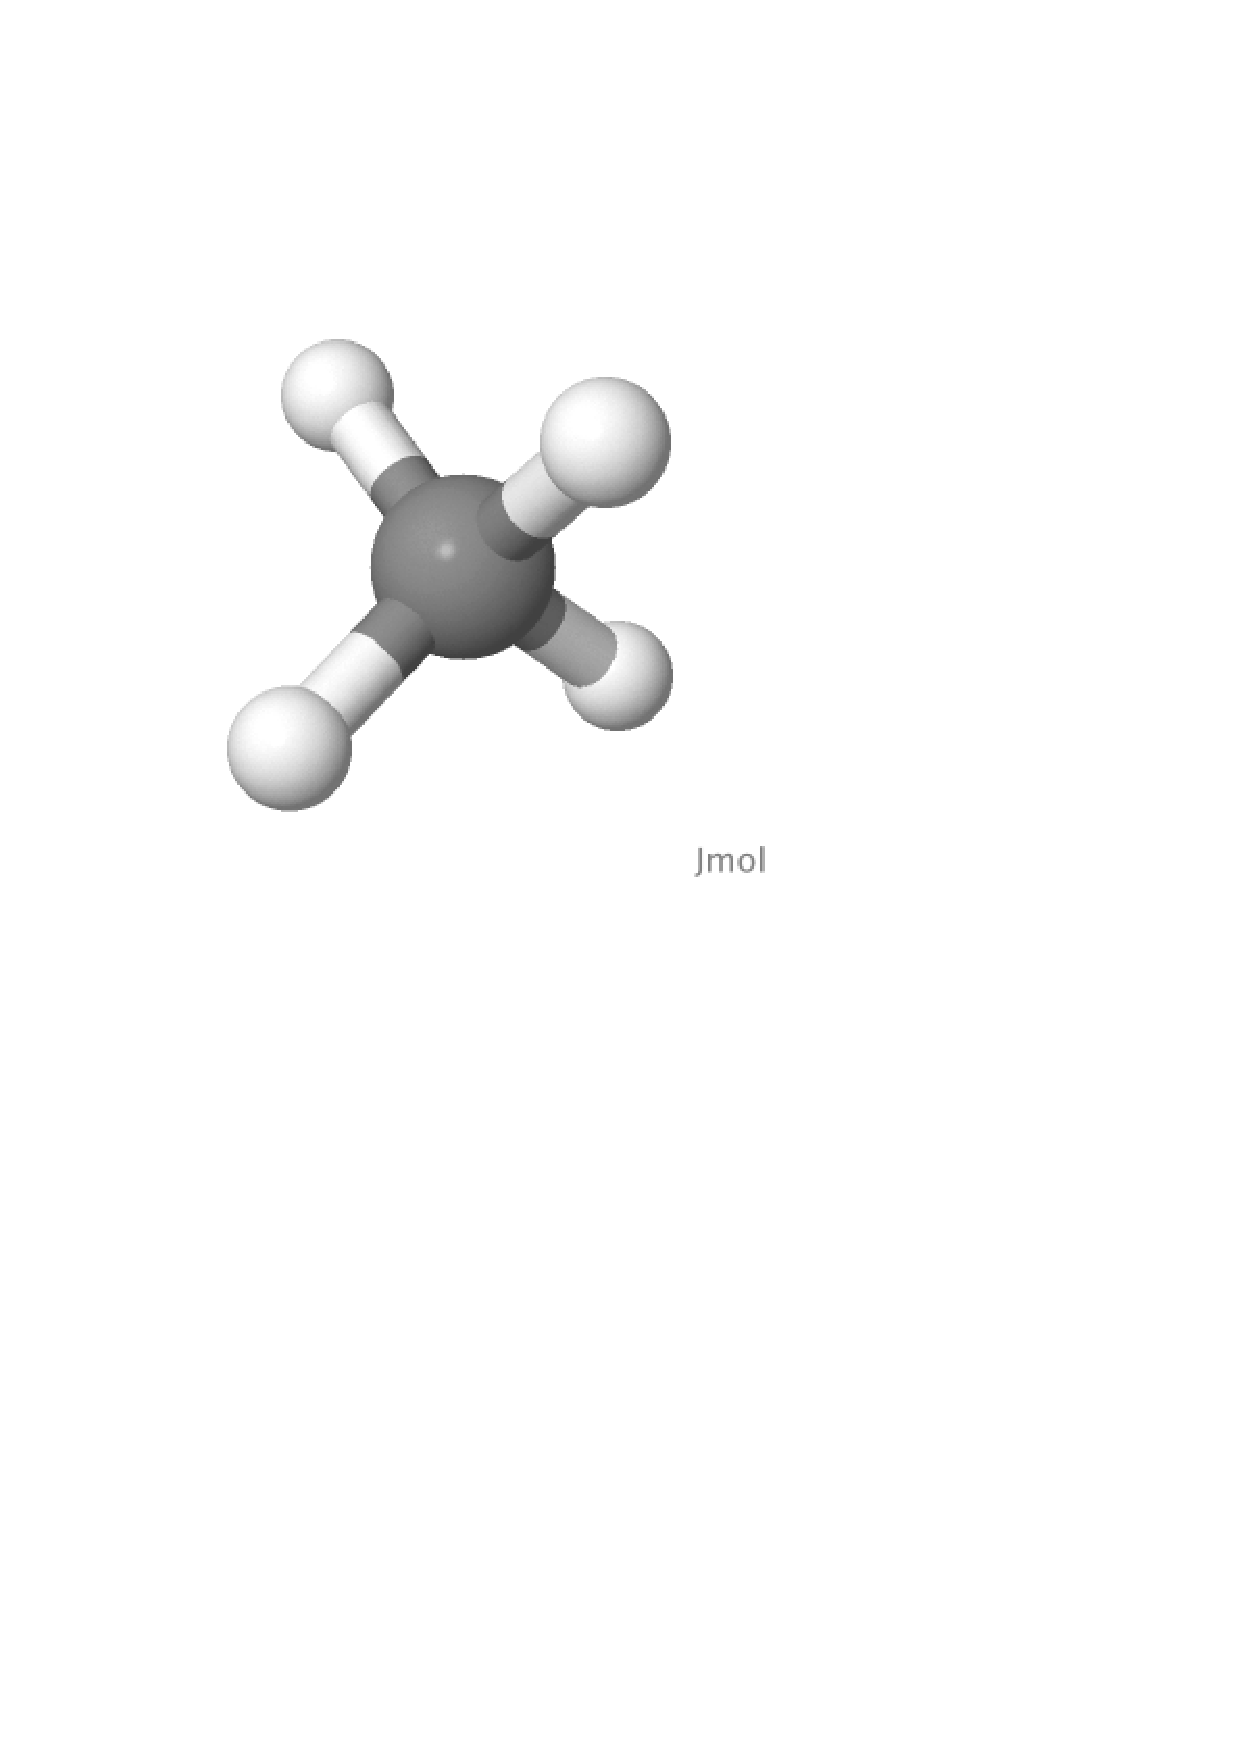
\includegraphics[scale=0.2, clip, viewport = 100 450 400 720]
        {figures/methane.pdf}
        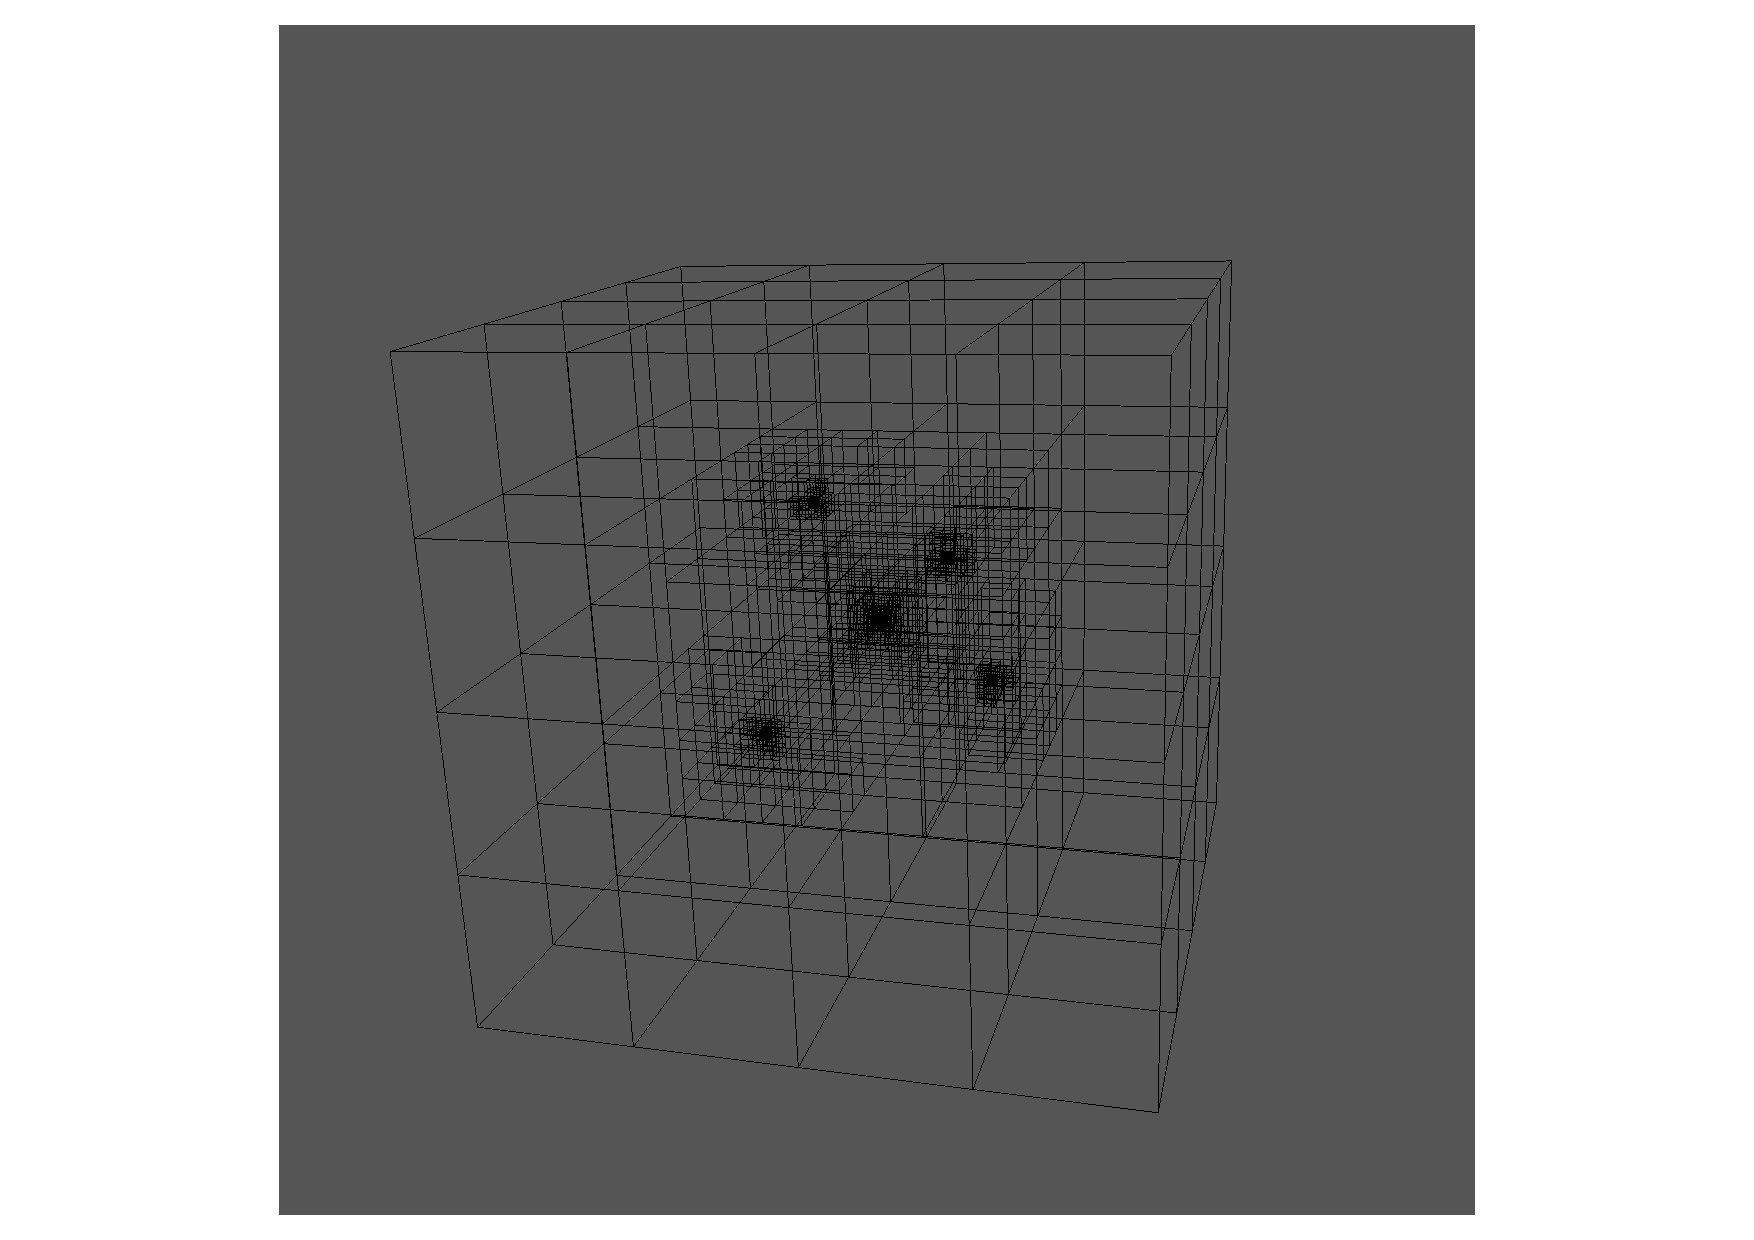
\includegraphics[scale=0.3, clip, viewport = 320 200 520 400]
        {figures/methaneGrid.pdf}
    \end{figure}

    \begin{figure}
        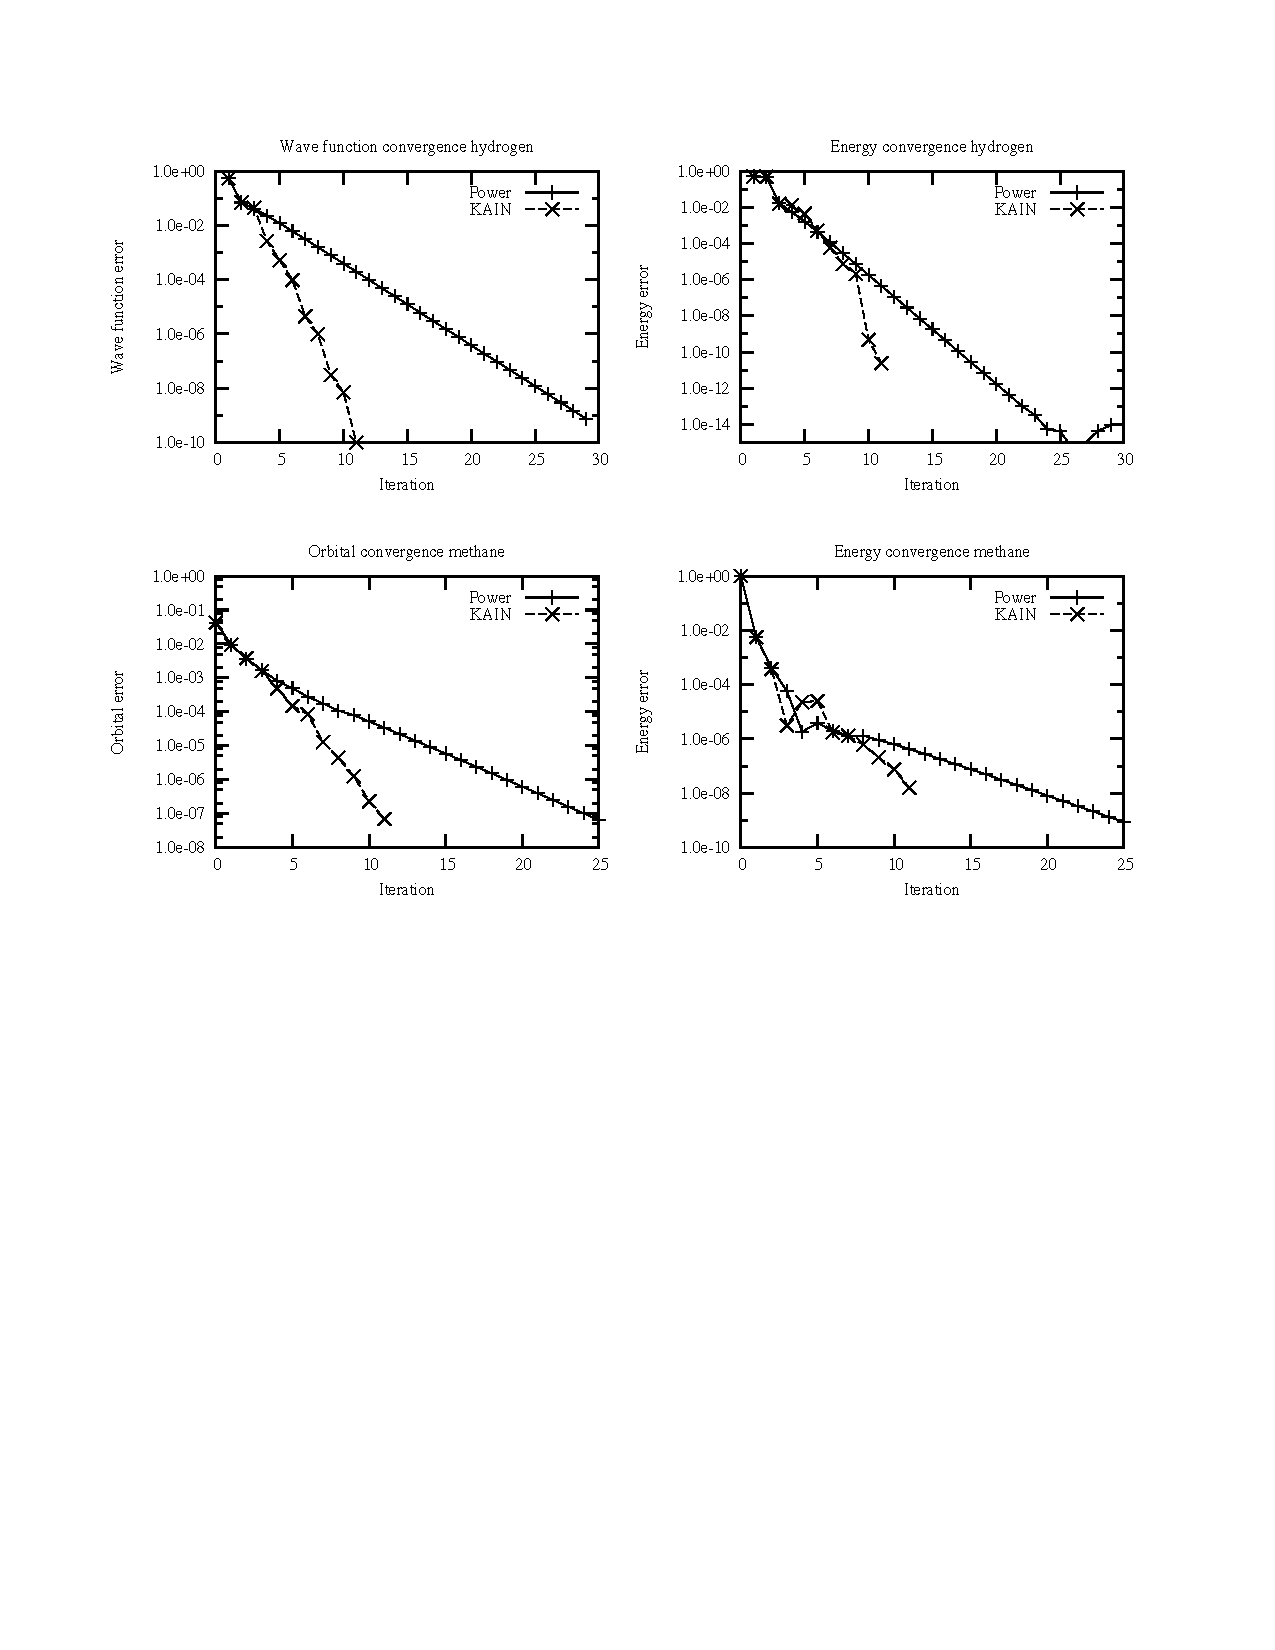
\includegraphics[scale=0.6, clip, viewport = 50 350 300 540]
        {figures/convergence.pdf}
    \end{figure}

    \end{column}
    \end{columns}
\end{frame}



\begin{frame}
    \frametitle{Orbital localization}
    \centering
    The Foster-Boys algorithm calculates the unitary transformation \\
    that maximizes the separation between orbitals by the measure
    \begin{equation}
	\nonumber
	L = \sum_{i}^{N_{occ}} \Big(
		\langle\phi_i|r_x|\phi_i\rangle^2 + 
		\langle\phi_i|r_y|\phi_i\rangle^2 + 
		\langle\phi_i|r_z|\phi_i\rangle^2 \Big)
    \end{equation}
    \begin{columns}
    \begin{column}[b]{0.48\linewidth}
    \begin{center}
    \only<1>{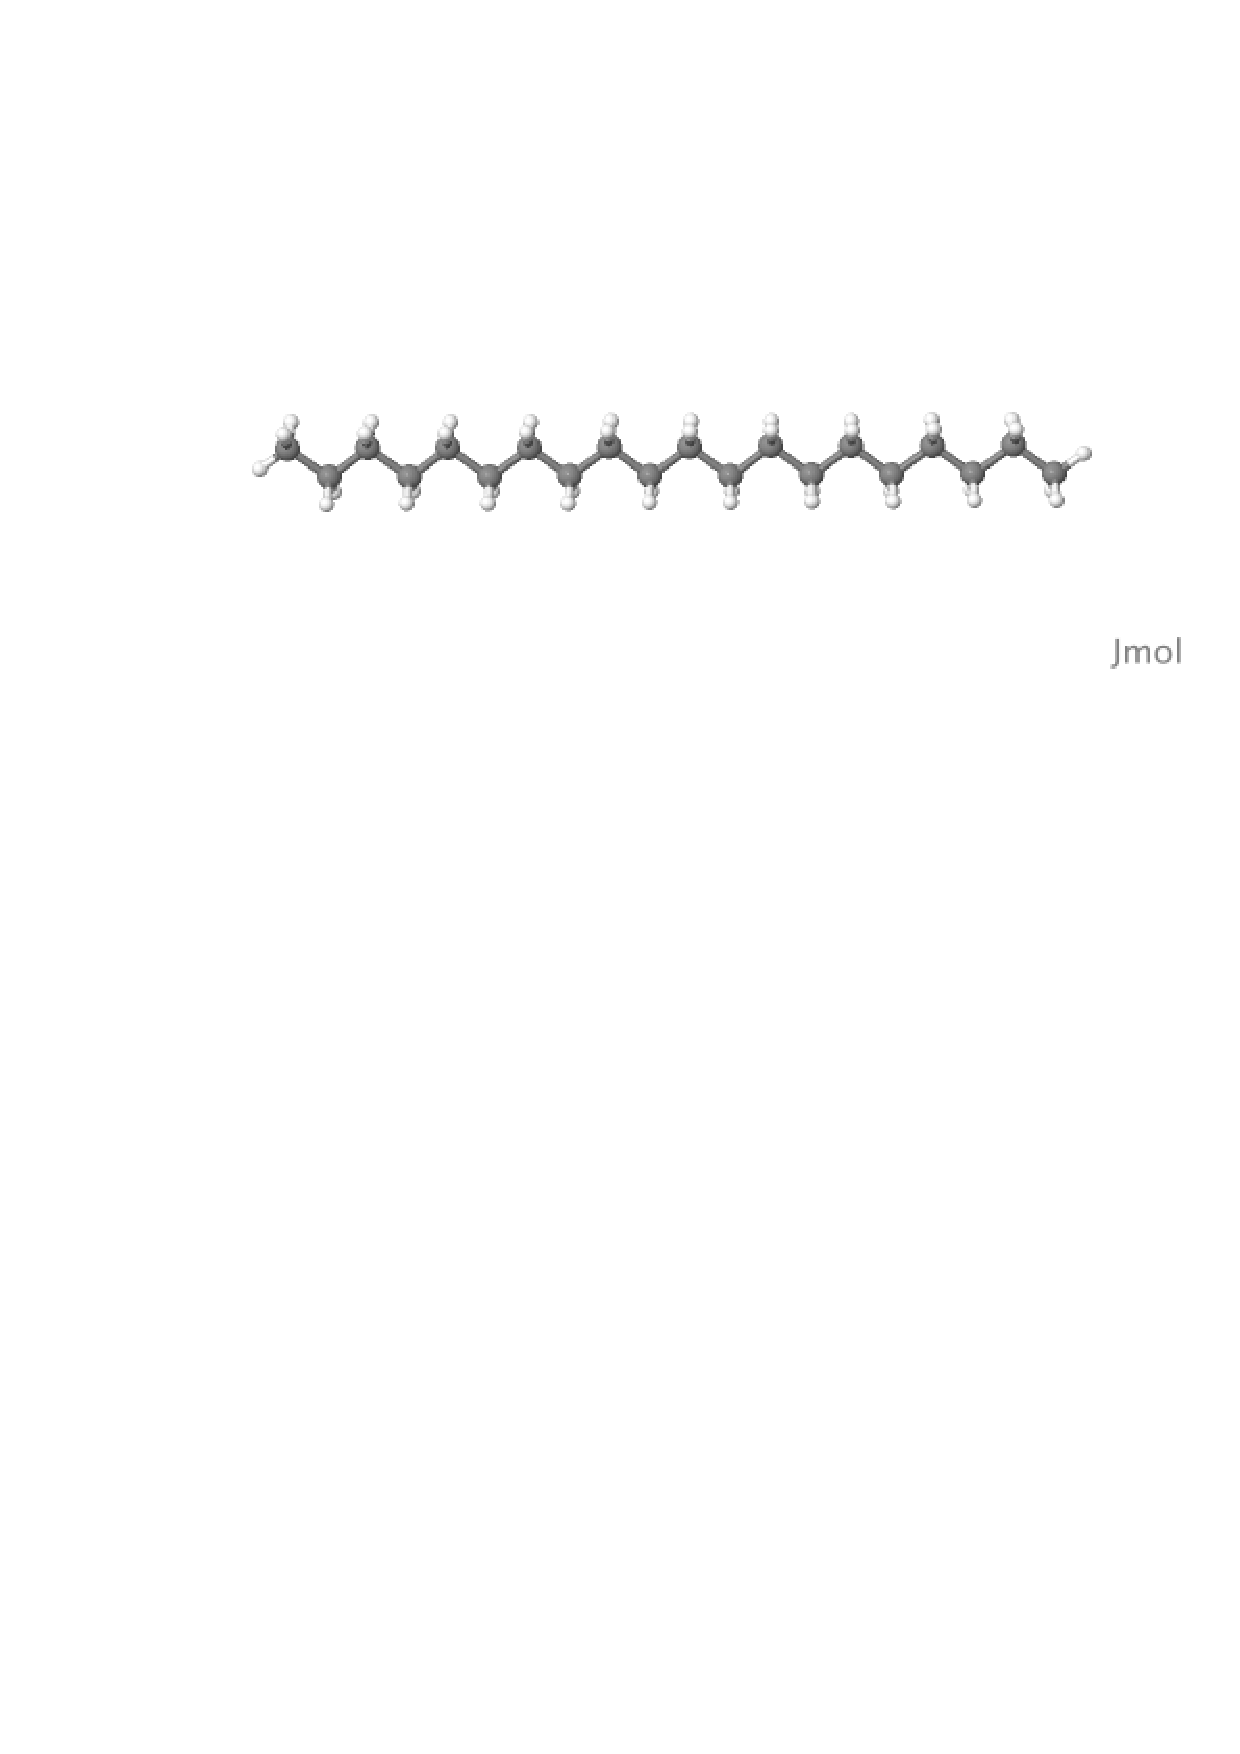
\includegraphics[scale=0.3, clip, viewport = 80 260 600 400]
        {figures/alkane.pdf}}
    \only<2,3>{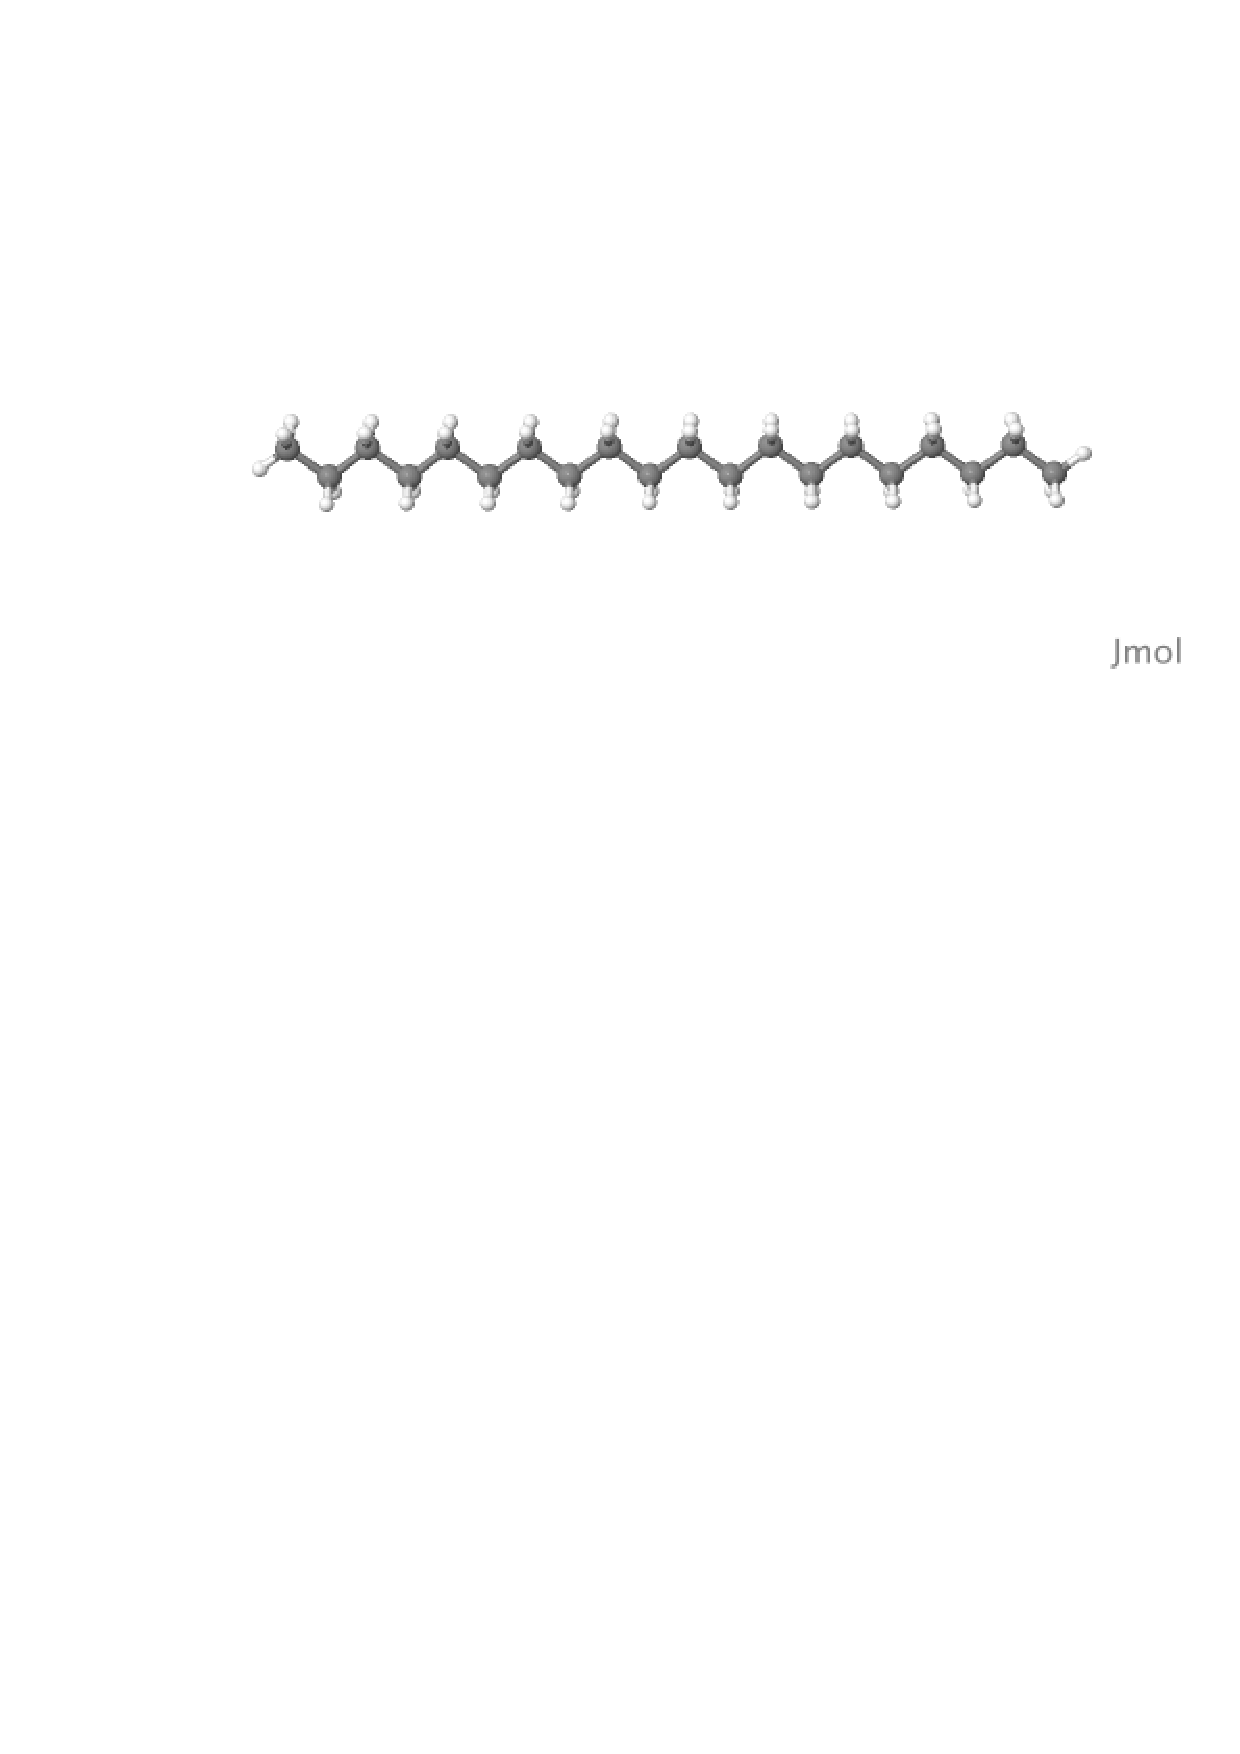
\includegraphics[scale=0.3, clip, viewport = 80 560 600 700]
        {figures/alkane.pdf}}
    \only<1>{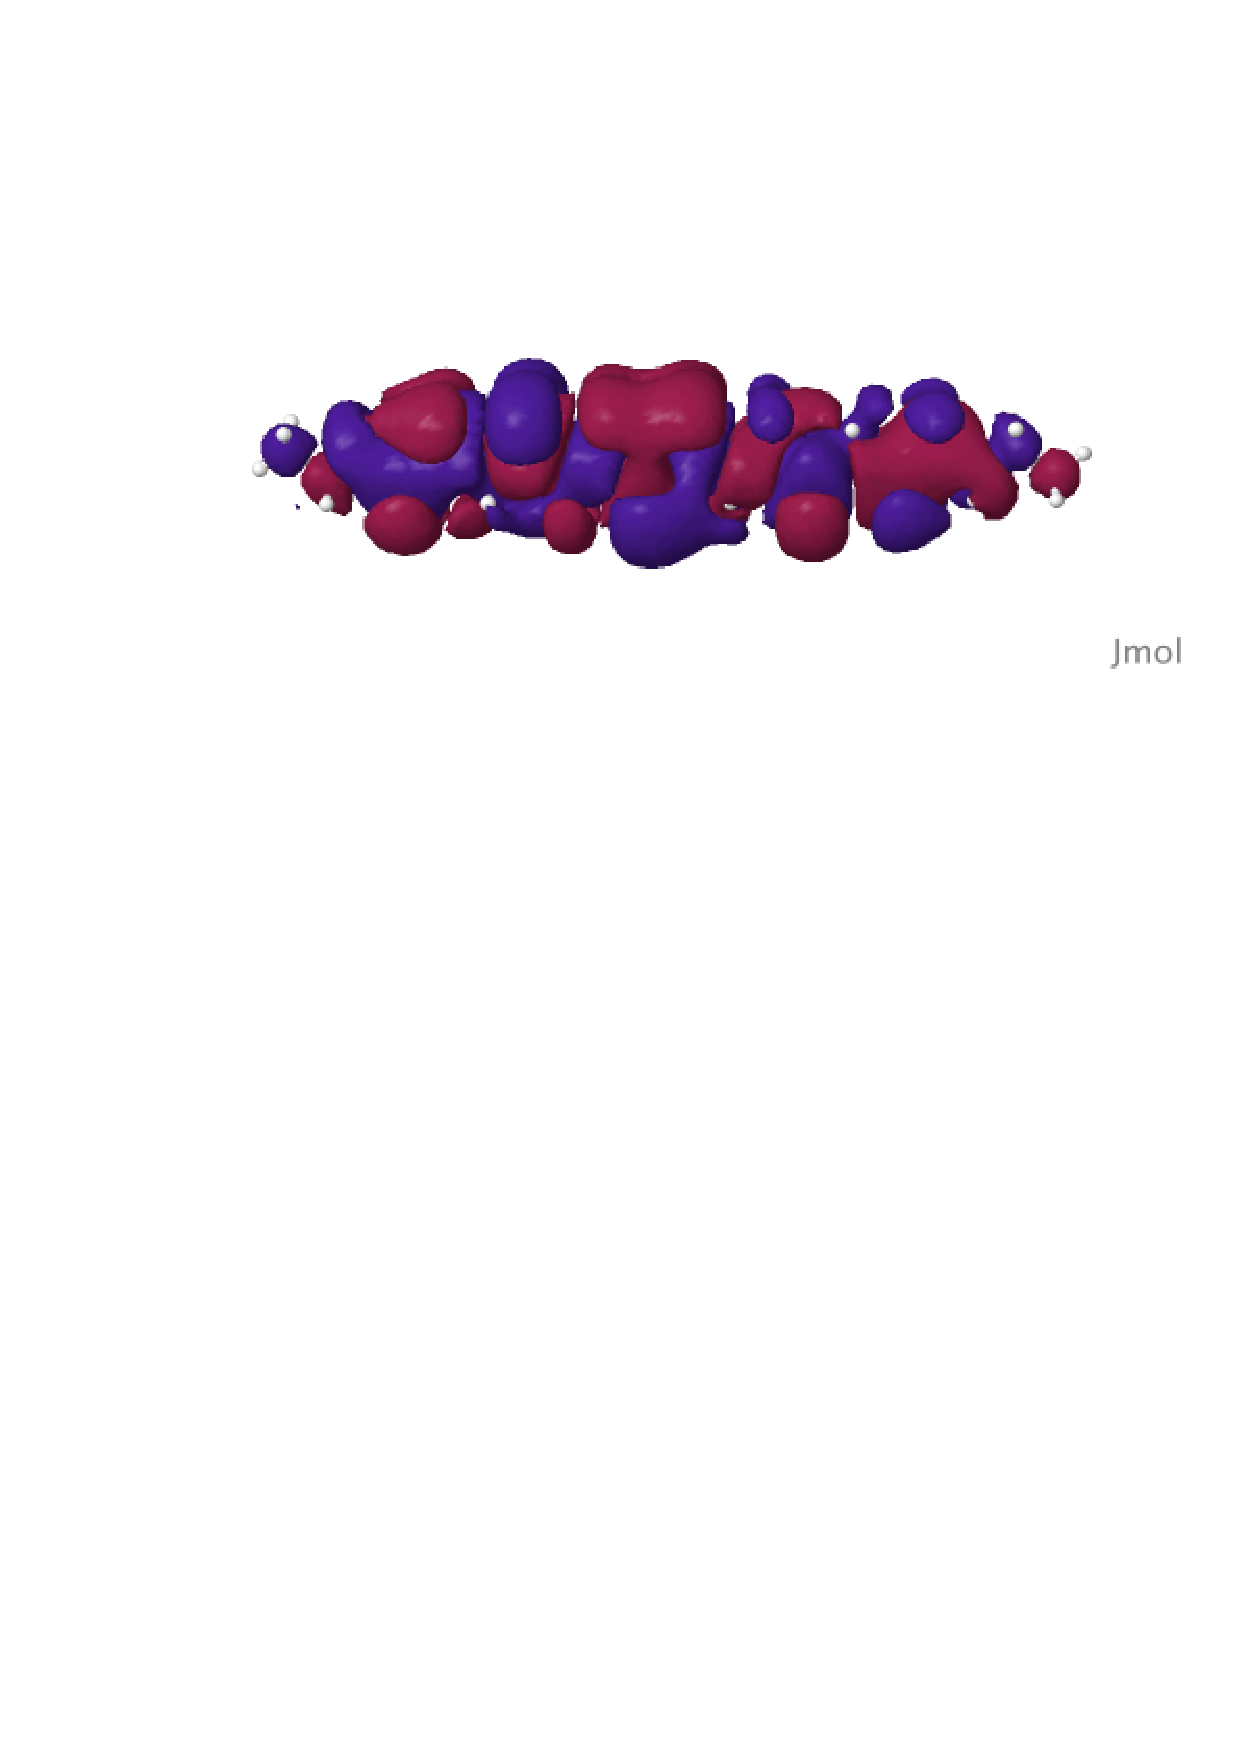
\includegraphics[scale=0.3, clip, viewport = 80 260 600 400]
        {figures/can_orb_1.pdf}}
    \only<2,3>{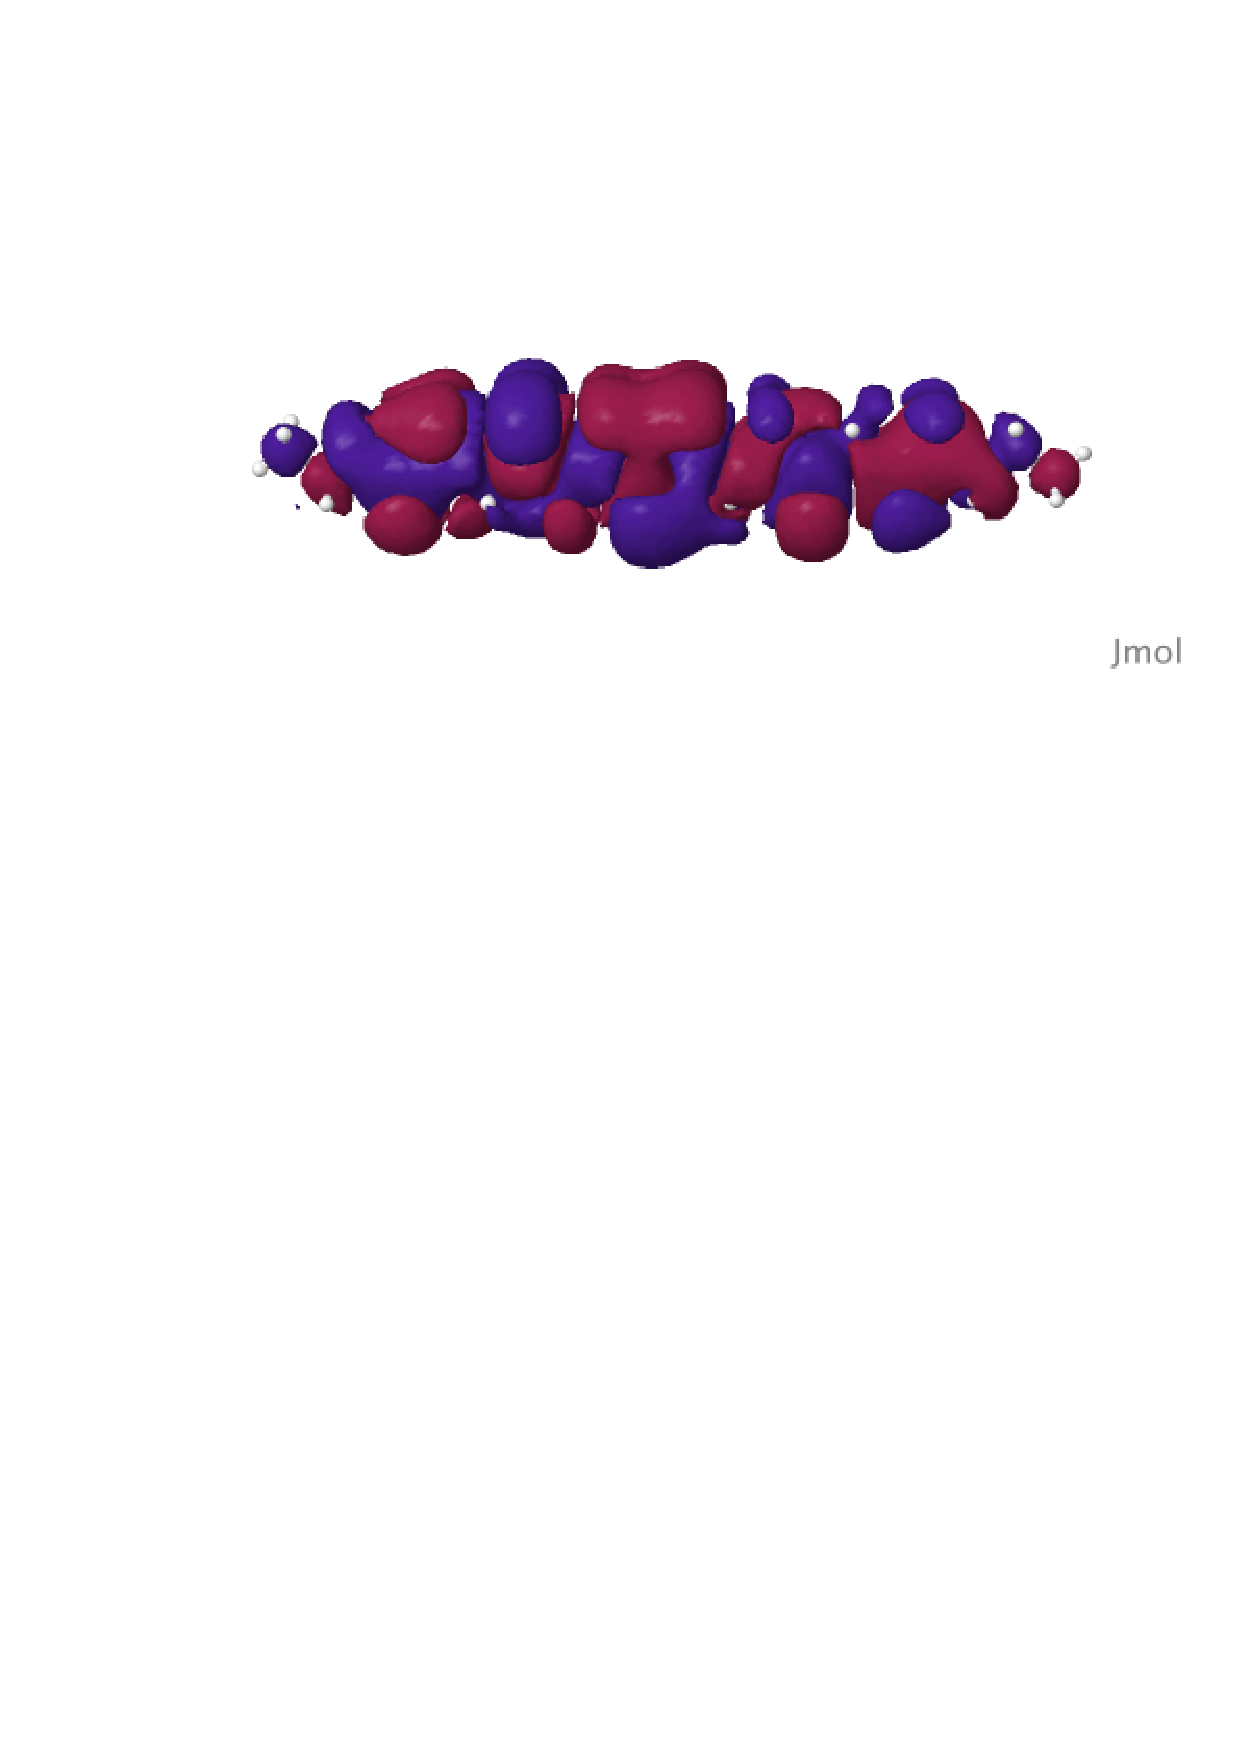
\includegraphics[scale=0.3, clip, viewport = 80 560 600 700]
        {figures/can_orb_1.pdf}}
    \only<1>{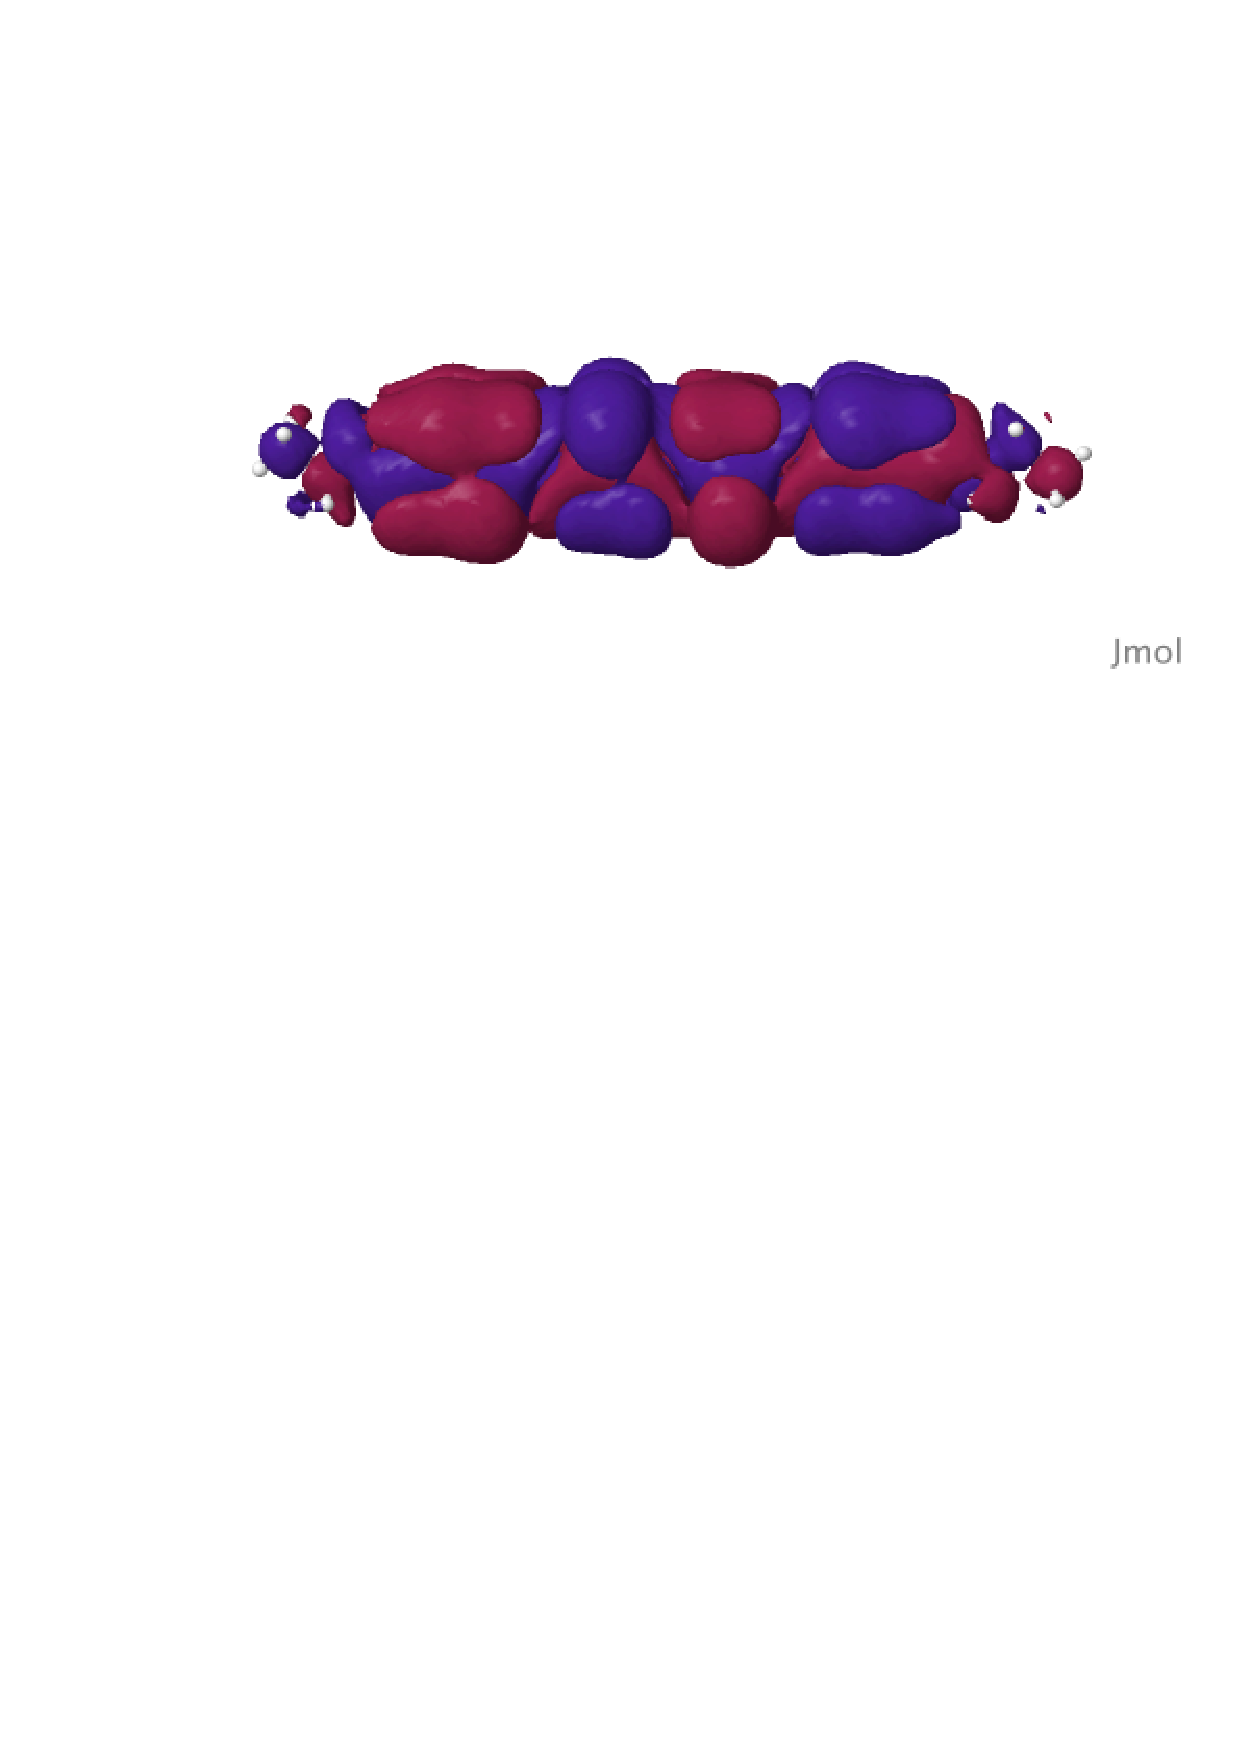
\includegraphics[scale=0.3, clip, viewport = 80 260 600 400]
        {figures/can_orb_2.pdf}}
    \only<2,3>{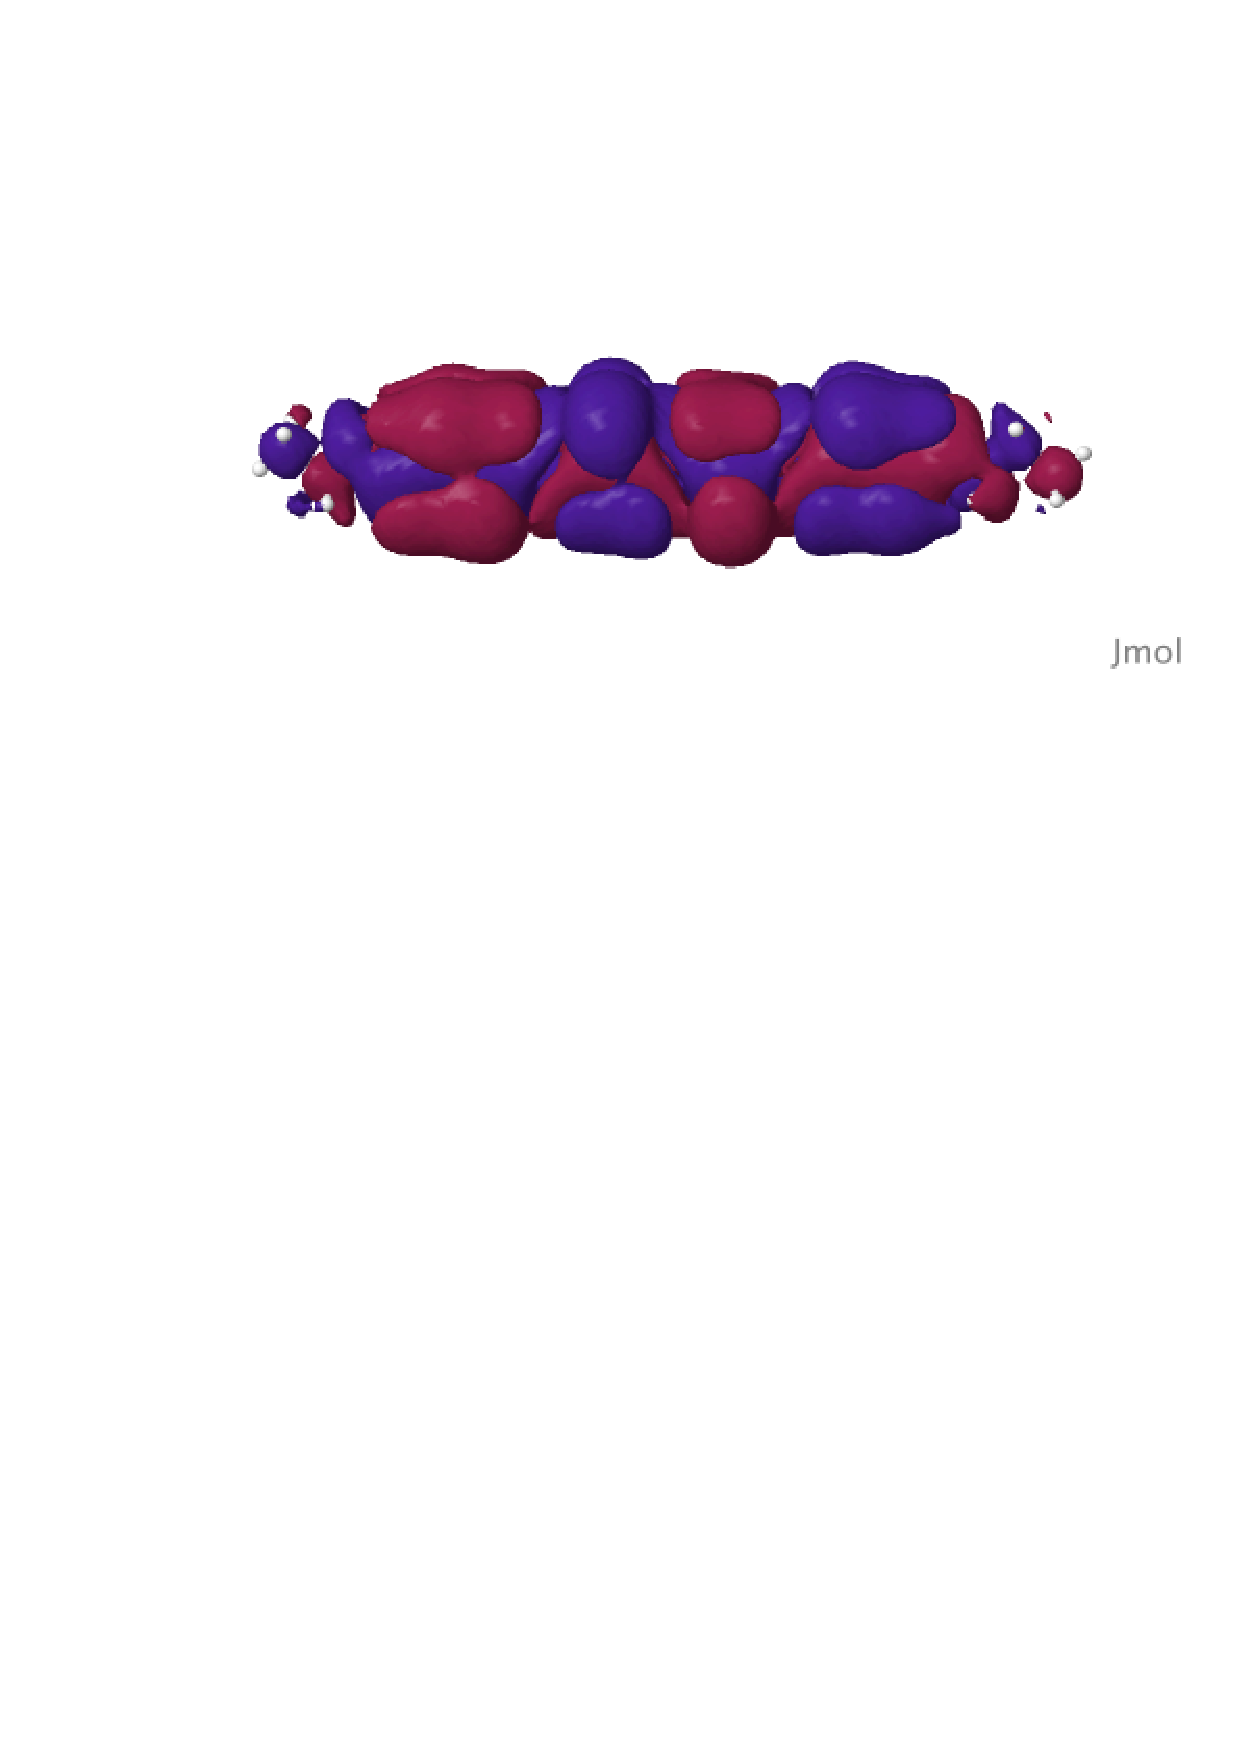
\includegraphics[scale=0.3, clip, viewport = 80 560 600 700]
        {figures/can_orb_2.pdf}}
    \end{center}
    \end{column}
    \begin{column}[b]{0.48\linewidth}
    \begin{center}
    \only<3>{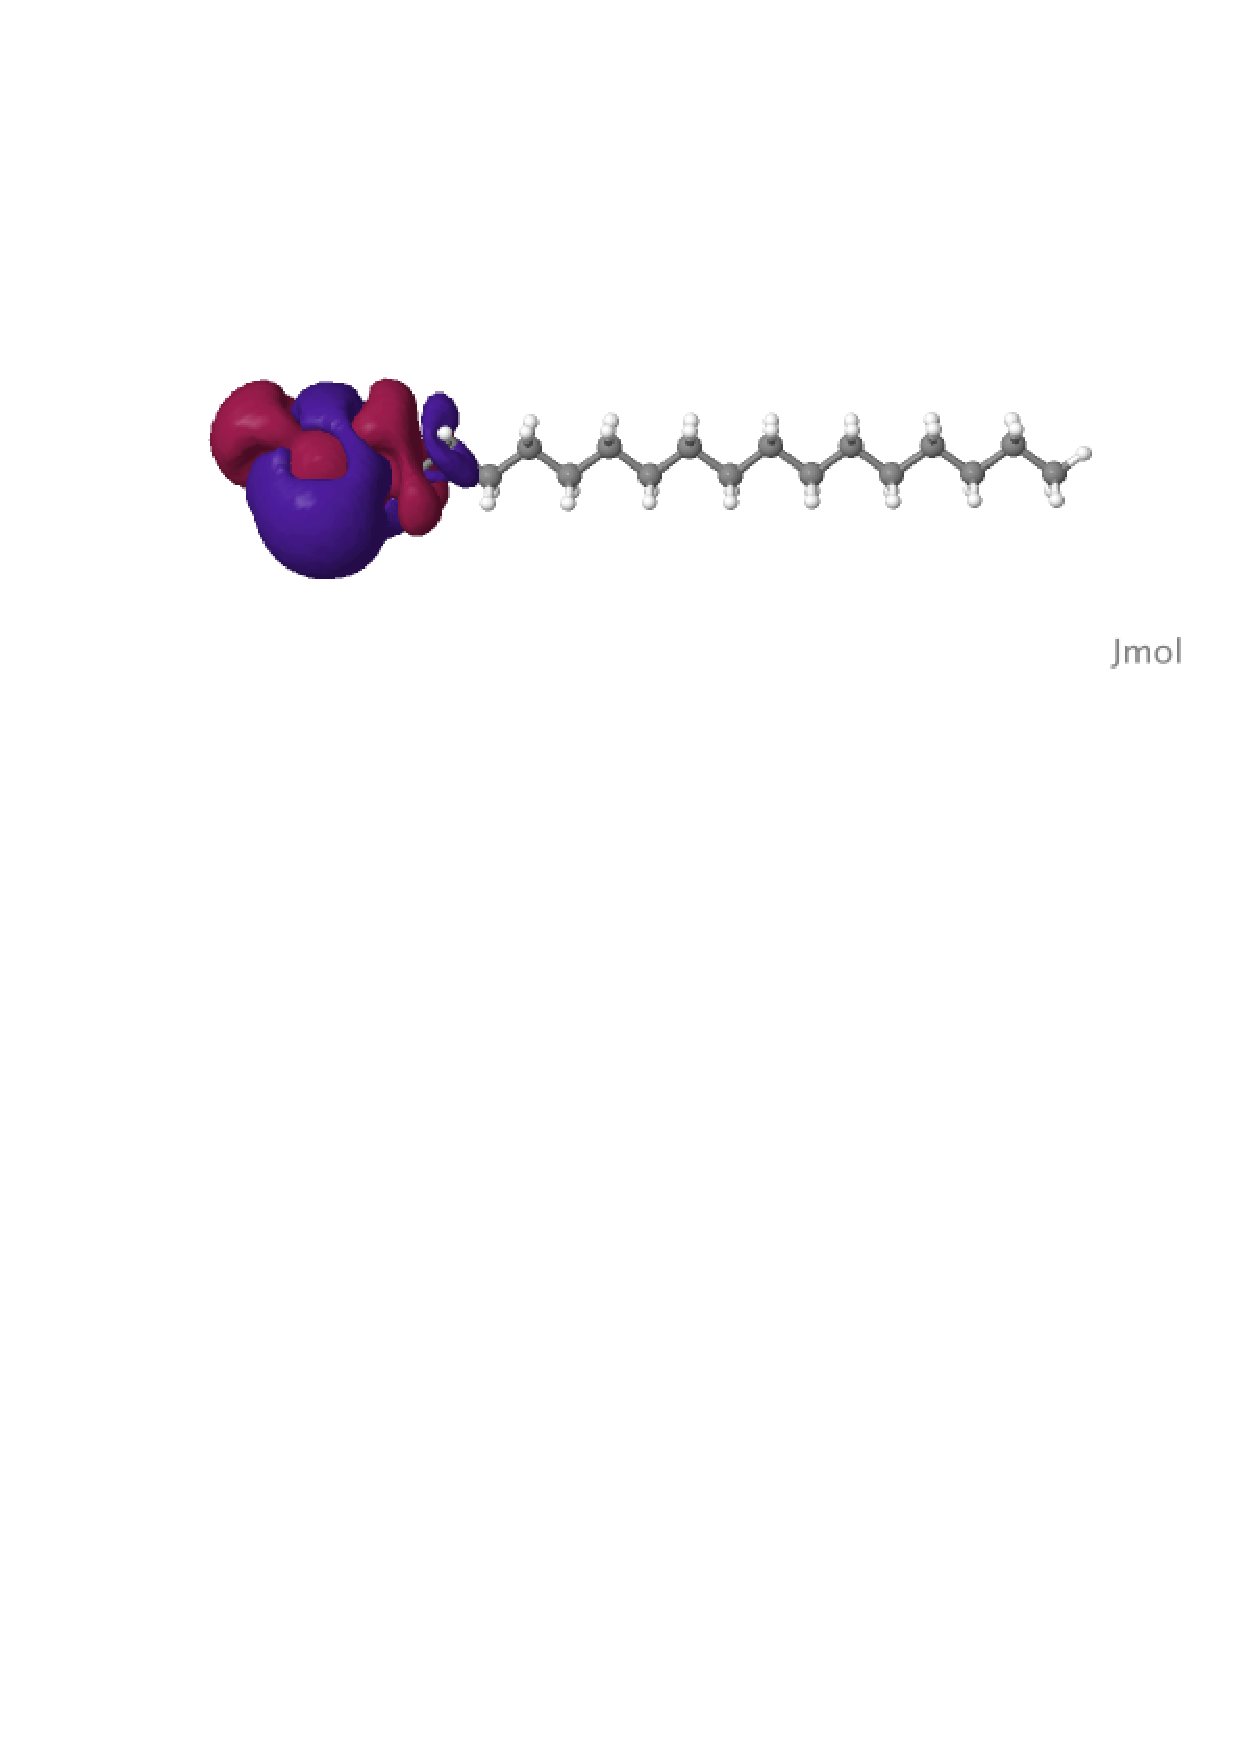
\includegraphics[scale=0.3, clip, viewport = 80 560 600 700]
        {figures/loc_orb_1.pdf}\\}
    \only<3>{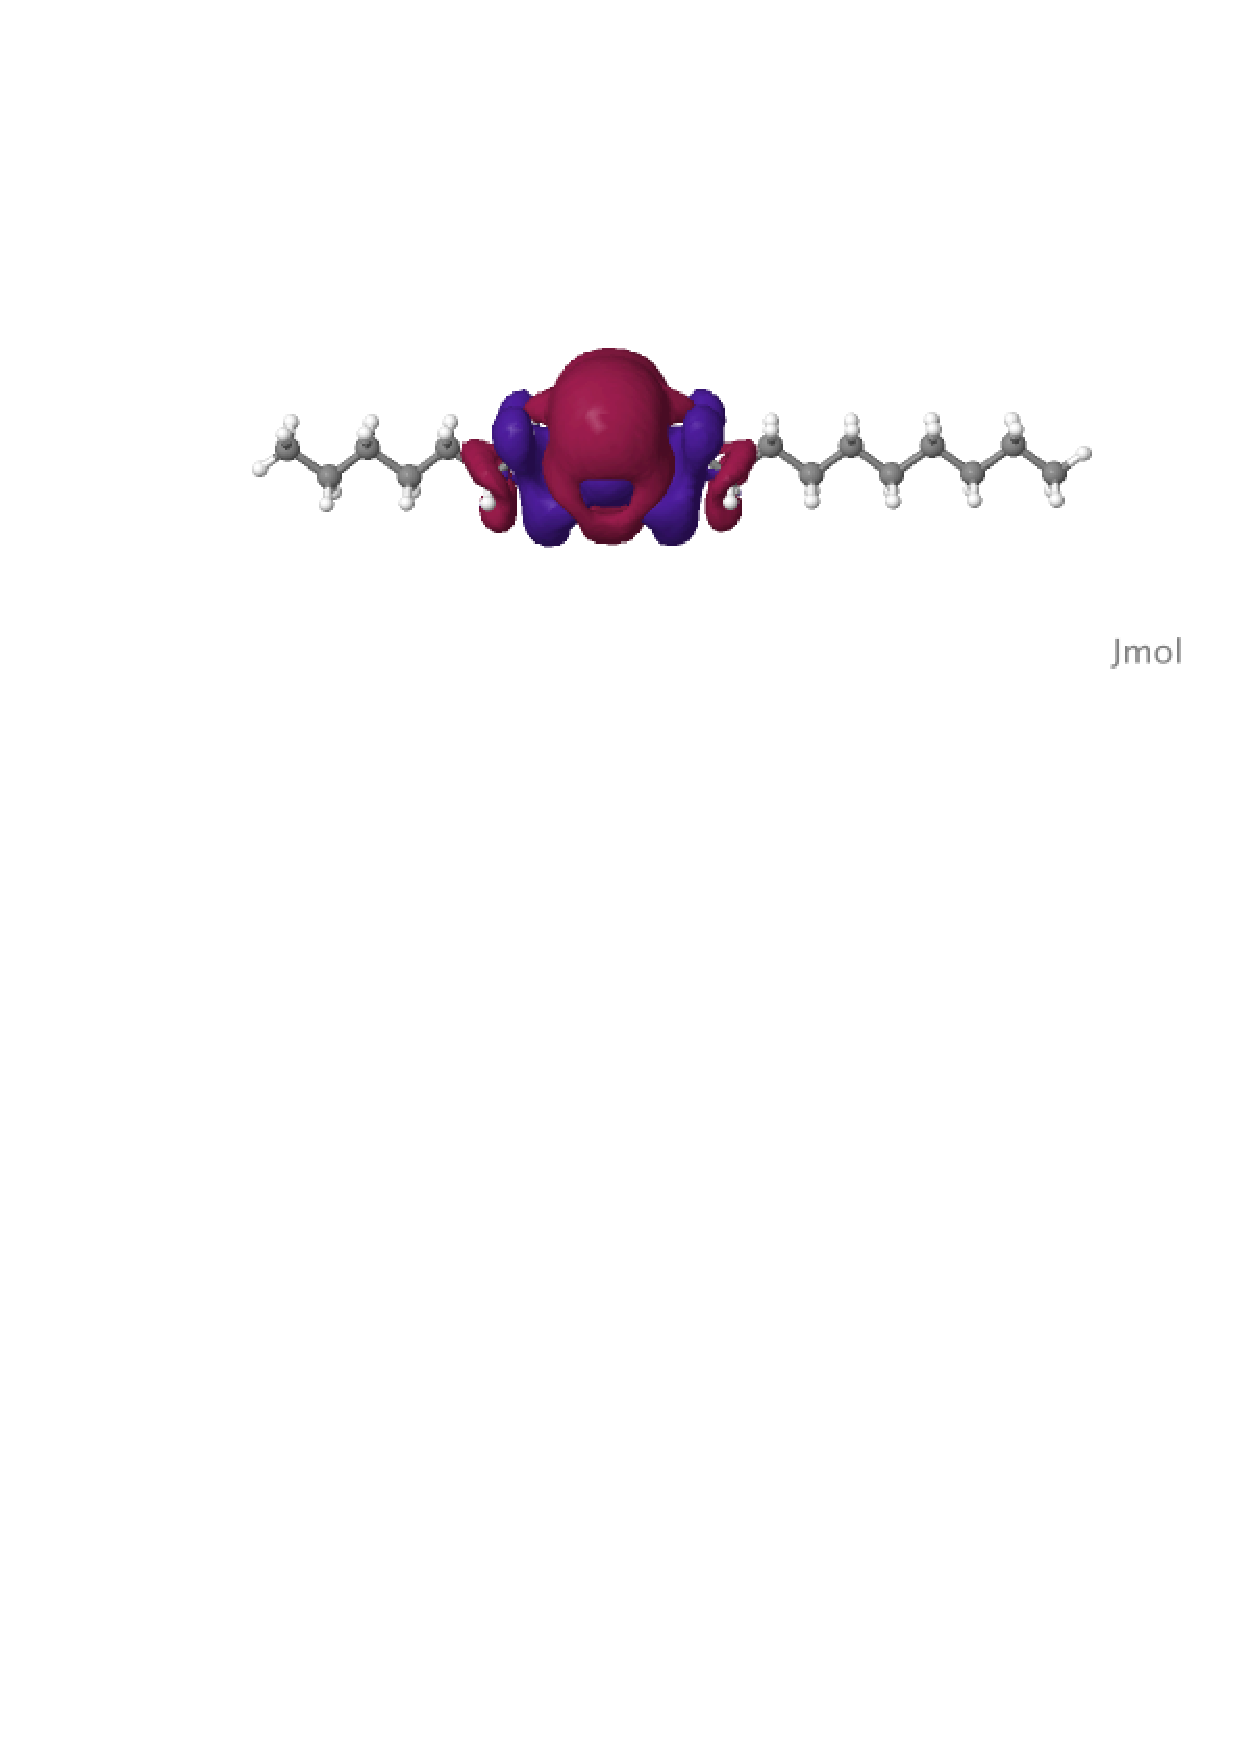
\includegraphics[scale=0.3, clip, viewport = 80 560 600 700]
        {figures/loc_orb_2.pdf}\\}
    \only<3>{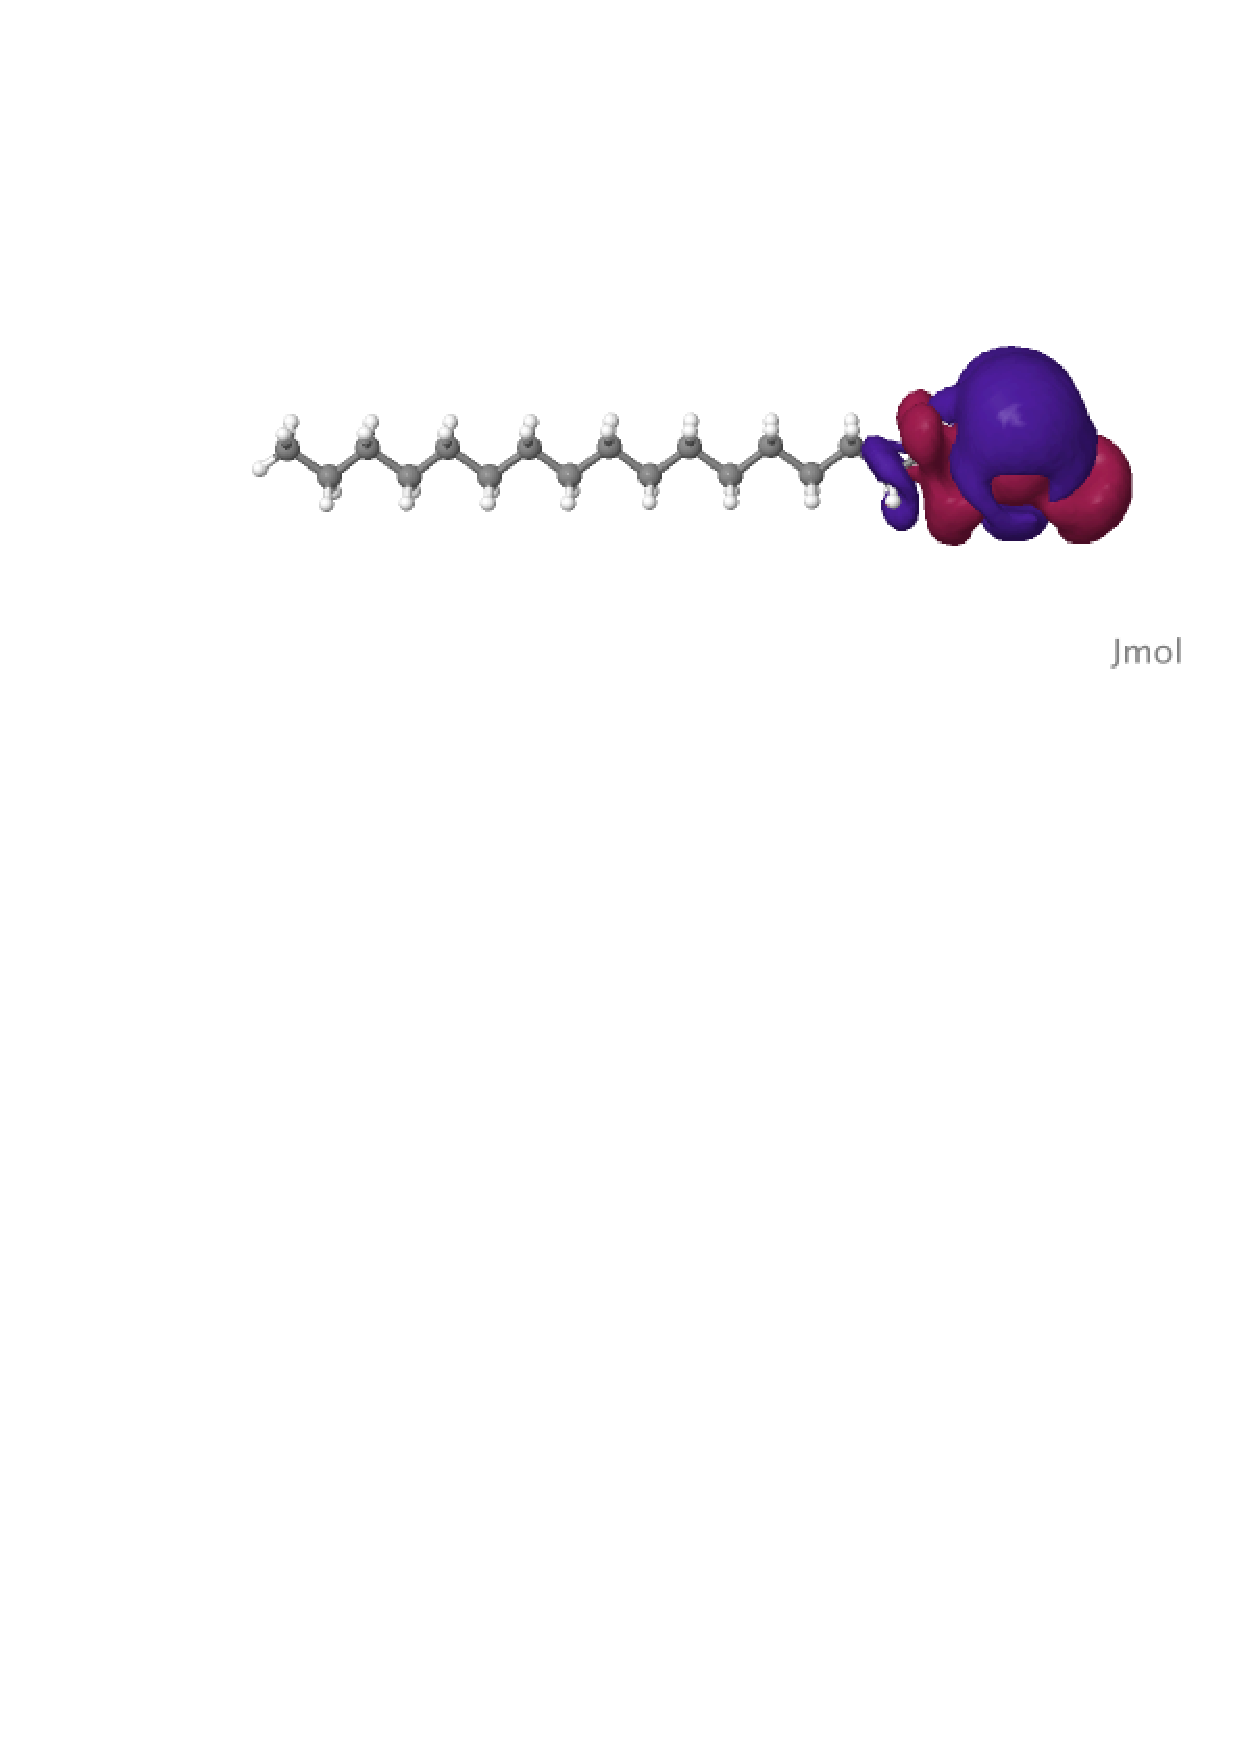
\includegraphics[scale=0.3, clip, viewport = 80 560 600 700]
        {figures/loc_orb_3.pdf}}
    \end{center}
    \end{column}
    \end{columns}
\end{frame}


\begin{frame}
    \frametitle{Calculation of Fock matrix}
    \begin{columns}
    \begin{column}[b]{0.55\textwidth}
    \centering
    We can solve directly for the localized MOs by introducing the
    (non-diagonal) Fock matrix into the HF/KS equations
    \begin{equation}
        \nonumber
        \phi_i^{n+1} =\ -2\hat{G}\left[\hat{V}^n\phi_i^n - 
            \sum_{j\neq i} F^n_{ij}\phi_j^n\right]
    \end{equation}

    \vspace{5mm}
    where we have the Fock matrix
    \begin{equation}
        \nonumber
        F_{ij} = \langle \phi_i | \hat{T} + \hat{V} | \phi_j \rangle
    \end{equation}

    \vspace{5mm}
    The kinetic part can be calculated using first order \\
    differential operators
    \begin{equation}
        \nonumber
        T_{ij} =
        \langle \phi_i | -\frac{1}{2}\nabla^2 | \phi_j \rangle = 
        \frac{1}{2}\langle \nabla \phi_i | \nabla \phi_j \rangle 
    \end{equation}

    \pause
    \vspace{5mm}
    or we can compute the (exact) Fock matrix at a given iteration without any 
    reference to the kinetic energy operator
    \begin{align}
        \nonumber
        F^{n+1} &= \tilde{S}^n F^{n} + \Delta F_{pot}^n\\
        \nonumber
        \tilde{S}^n &= \langle \phi_i^{n+1} | \phi_j^n \rangle\\
        \nonumber
        \Delta F_{pot}^n
        &= \langle \phi_i^{n+1} | \hat{V}^n | \Delta\phi_j^n \rangle
        + \langle \phi_i^{n+1} | \Delta\hat{V}^n | \phi_j^n \rangle
    \end{align}

    \end{column}

    \begin{column}[b]{0.45\textwidth}
    \begin{figure}
	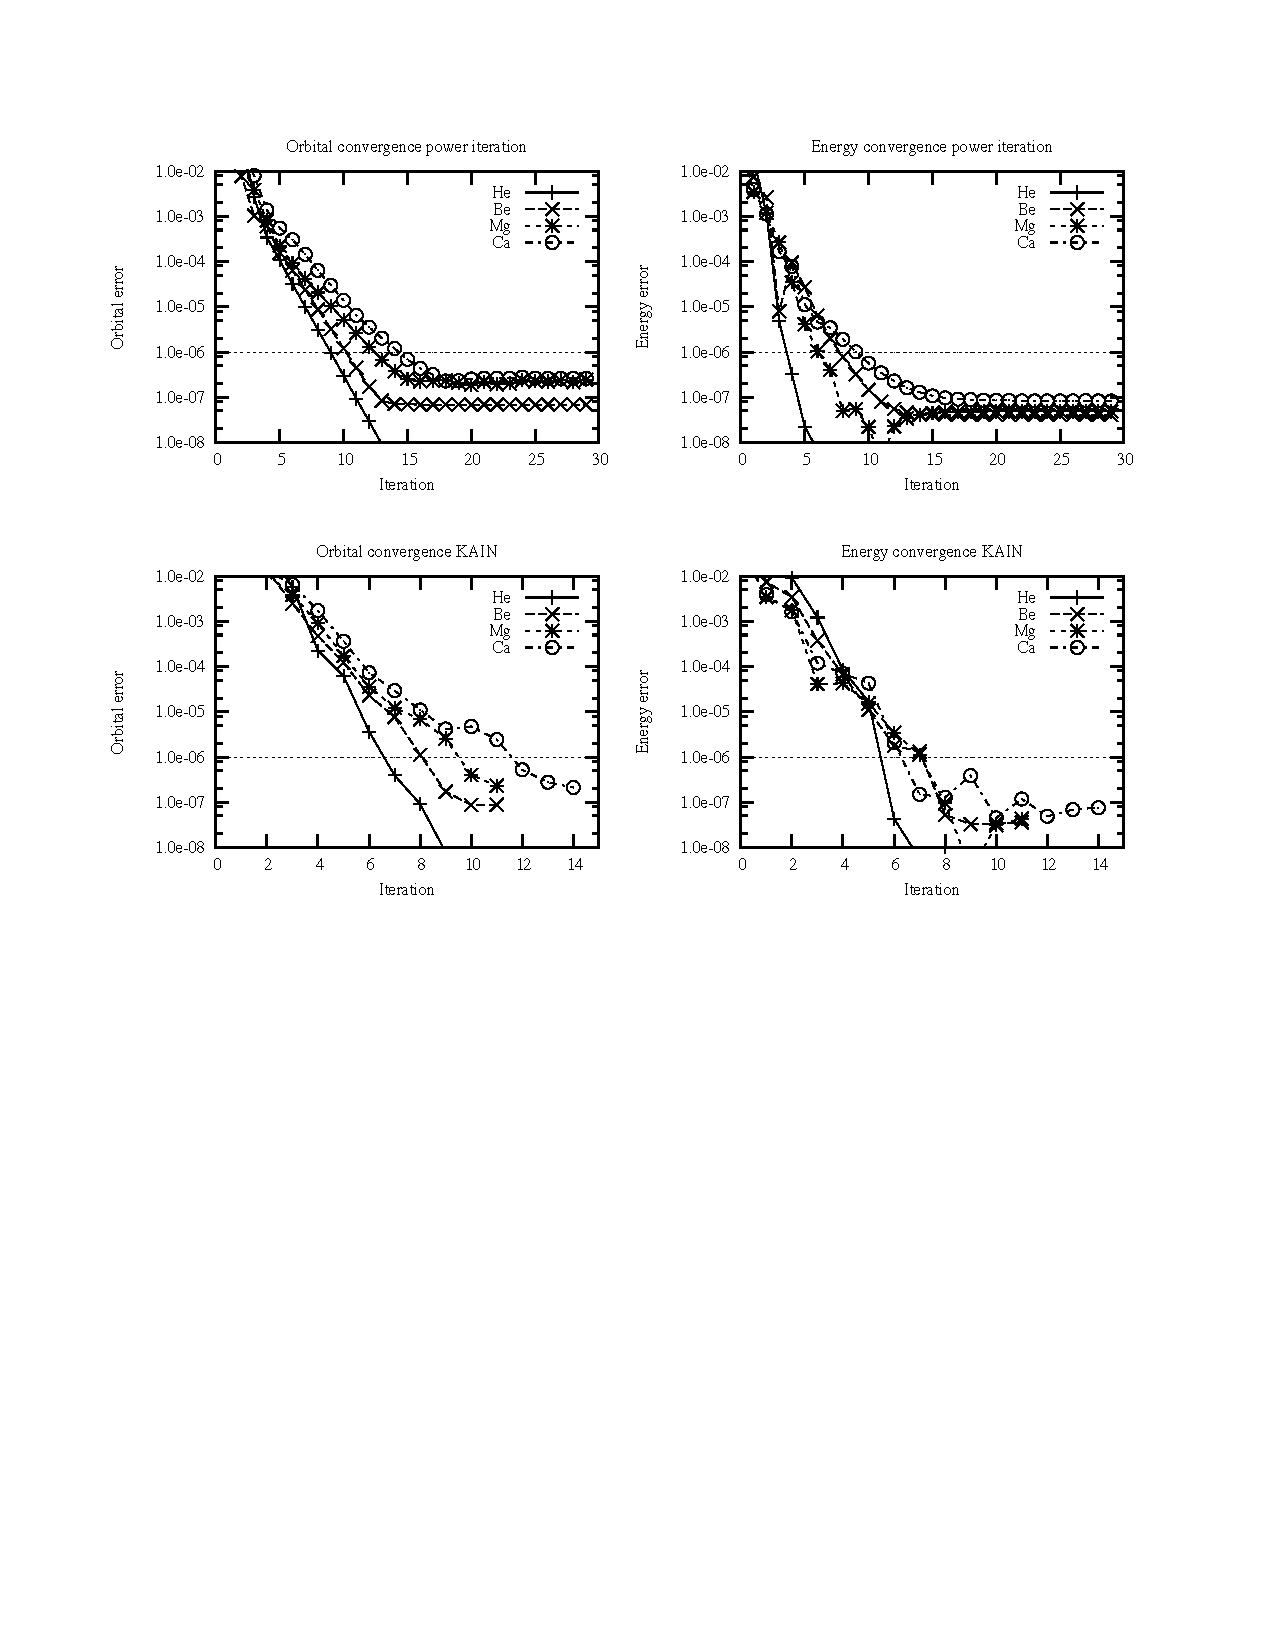
\includegraphics[scale=0.5, clip, viewport = 50 550 300 740]
                {figures/accuracy.pdf}
    \end{figure}
    \begin{figure}
	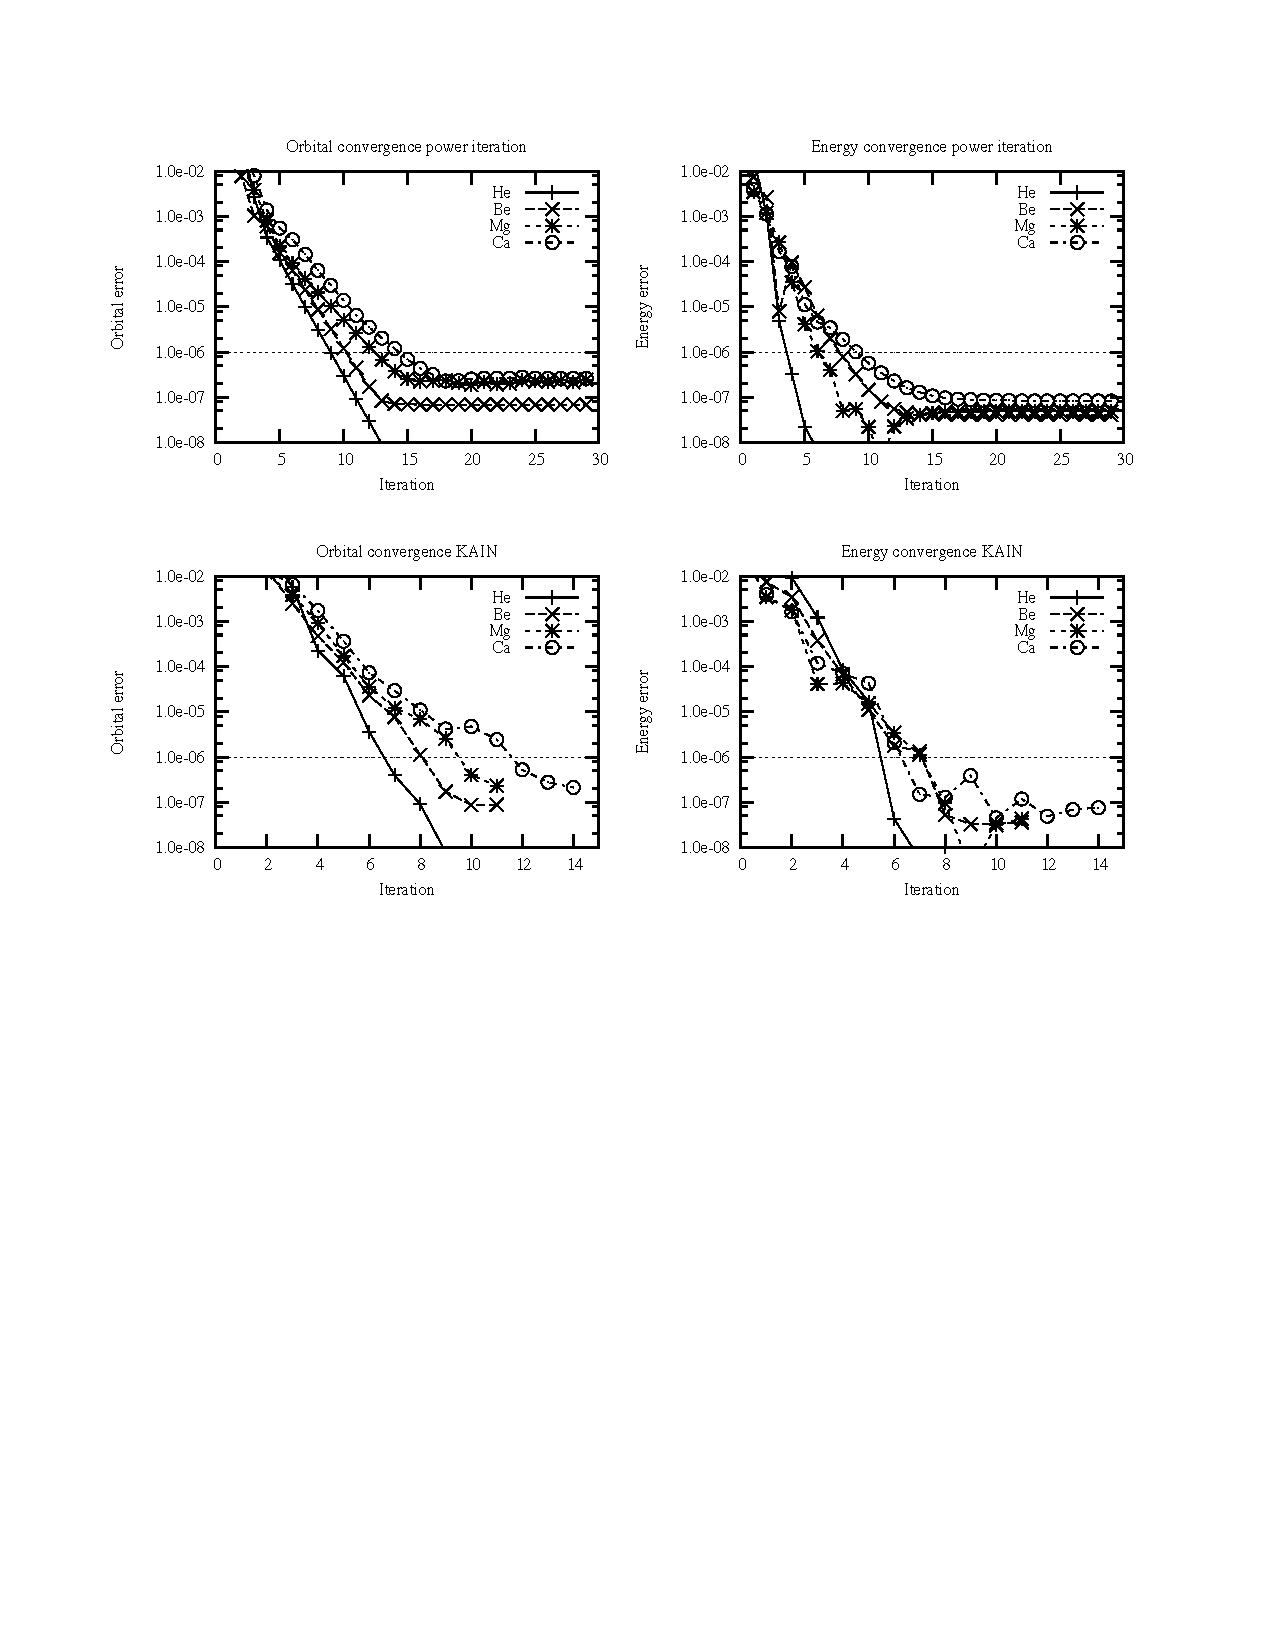
\includegraphics[scale=0.5, clip, viewport = 300 550 550 740]
                {figures/accuracy.pdf}
    \end{figure}

    \end{column}
    \end{columns}
\end{frame}


%\begin{frame}
%    \frametitle{Hydrogen atom}
%    \centering
%    \textbf{Power iteration}
%    \begin{equation}
%	\nonumber
%	\phi^{n+1} = -2\hat{H}\left[v_{nuc}\phi^n\right]
%    \end{equation}
%    \ \\
%    \ \\
%    \ \\
%    \begin{columns}
%    \begin{column}{.10\textwidth}
%    \ \\
%    \end{column}
%    \begin{column}{.40\textwidth}
%    \centering
%    \textbf{Orbital update}
%    \begin{equation}
%	\nonumber
%	\Delta\phi^n = \phi^{n+1} - \phi^n
%    \end{equation}
%    \end{column}
%    \begin{column}{.50\textwidth}
%    \centering
%    \textbf{Energy update}
%    \begin{equation}
%	\nonumber
%	\Delta \epsilon^n = \left<\phi^{n+1}|v_{nuc}|\Delta\phi^n\right>
%    \end{equation}
%    \end{column}
%    \end{columns}    
%    \begin{center}
%	\includegraphics[scale=0.6, clip, viewport = 50 550 540 730]
%       {figures/convergence.pdf}
%    \end{center}
%\end{frame}

%\begin{frame}
%    \frametitle{Hydrogen atom}
%    \only<1>{\includegraphics[viewport = 50 430 300 640, clip, scale=1.2]
%       {figures/s1Orb_1.pdf}}
%    \only<2>{\includegraphics[viewport = 50 430 300 640, clip, scale=1.2]
%       {figures/s1Orb_2.pdf}}
%    \only<3>{\includegraphics[viewport = 50 430 300 640, clip, scale=1.2]
%       {figures/s1Orb_3.pdf}}
%    \only<4>{\includegraphics[viewport = 50 430 300 640, clip, scale=1.2]
%       {figures/s1Orb_4.pdf}}
%    \only<5>{\includegraphics[viewport = 50 430 300 640, clip, scale=1.2]
%       {figures/s1Orb_5.pdf}}
%    \only<6>{\includegraphics[viewport = 50 430 300 640, clip, scale=1.2]
%       {figures/s1Orb_10.pdf}}
%\end{frame}

%\begin{frame}
%    \frametitle{Many-electron systems}
%    \begin{columns}
%    \begin{column}[b]{0.1\textwidth}
%    \ \\
%    \end{column}
%    \begin{column}[b]{0.4\textwidth}
%    \centering
%    Density
%    \begin{equation}
%	\nonumber
%	\rho^n(\boldsymbol{r}) = \sum_i |\phi_i^n(\boldsymbol{r})|^2
%    \end{equation}
%    \end{column}
%    \begin{column}[b]{0.4\textwidth}
%    \centering
%    Potentials
%    \begin{equation}   
%	\nonumber
%	\rho^n(\boldsymbol{r}) \rightarrow v_{eff}^n(\boldsymbol{r})
%    \end{equation}
%    \end{column}
%    \begin{column}[b]{0.1\textwidth}
%    \ \\
%    \end{column}
%    \end{columns}
%    \ \\
%    \ \\
%    \begin{columns}
%    \begin{column}[b]{0.1\textwidth}
%    \ \\
%    \end{column}
%    \begin{column}[b]{0.4\textwidth}
%    \centering
%    Power iteration
%    \begin{equation}
%	\nonumber
%	\tilde{\phi}_i^n = -2\hat{H}\left[v_{eff}^n\phi_i^n\right]
%    \end{equation}
%    \end{column}
%    \begin{column}[b]{0.4\textwidth}
%    \centering
%    Calculate updates
%    \begin{equation}
%	\nonumber
%	\Delta\phi^n = \tilde{\phi}^n - \phi^n
%    \end{equation}
%    \end{column}
%    \begin{column}[b]{0.1\textwidth}
%    \ \\
%    \end{column}
%    \end{columns}
%    \ \\
%    \ \\
%    \pause
%    \only<1,2>{
%    \centering
%    \ \\
%    \textbf{Complicating issues}
%    \ \\
%    \begin{columns}
%    \begin{column}[b]{0.25\textwidth}
%    \ \\
%    \end{column}
%    \begin{column}[b]{0.75\textwidth}
%    \begin{itemize}
%	\item	Straightforward iteration will bring all\\ 
%		orbitals to the lowest energy eigenfunction
%	\item	Orthonormality must be imposed
%	\item	Achieved by diagonalizing the Fock matrix 
%    \end{itemize}
%    \end{column}
%    \end{columns}
%    \begin{equation}
%        \nonumber
%        F_{ij} = \left<\phi_i|\hat{T} + v_{eff}|\phi_j\right>
%    \end{equation}
%    \ \\
%    \ \\
%    \ \\
%    \ \\
%    }
%    \only<3,4,5>{
%    \centering
%    Compute Fock matrix update
%    \begin{equation}
%	\nonumber
%	\Delta F_{ij}^n = \left<\tilde{\phi}_i^n|v_{eff}^n |\Delta\phi_j^n\right>
%			    + \left<\tilde{\phi}_i^n|\Delta v_{eff}^n|\phi_j^n\right>
%    \end{equation}
%    \ \\
%    \ \\
%    \ \\
%    \pause
%    \pause
%    \begin{columns}
%    \begin{column}[b]{0.1\textwidth}
%    \ \\
%    \end{column}
%    \begin{column}[b]{0.4\textwidth}
%    \centering
%    Diagonalize matrix
%    \begin{equation}
%	\nonumber
%	F^{n+1} = M^{-1}\tilde{F}^nM
%    \end{equation}
%    \end{column}
%    \begin{column}[b]{0.4\textwidth}
%    \centering
%    Rotate orbitals
%    \begin{equation}
%	\nonumber
%	\phi_i^{n+1} = \sum_jM^{-1}_{ij}\tilde{\phi}_j^n
%    \end{equation}
%    \end{column}
%    \begin{column}[b]{0.1\textwidth}
%    \ \\
%    \end{column}
%    \end{columns}
%    \ \\
%    \ \\
%    \pause
%    Compute iterative subspace acceleration (KAIN or DIIS)\\
%    \ \\
%    Orthonormalize\\
%    \ \\
%    }
%\end{frame}

\begin{frame}
\frametitle{Accurate calculations}
\centering
LDA energies in atomic units (Hartree)
\begin{table}
    \tiny
    \centering
    \begin{tabular}{lr@{.}lr@{.}lr@{.}lr@{.}lr@{.}lr@{.}l}
    \hline
    \hline
    &\multicolumn{4}{c}{Helium}
    &\multicolumn{4}{c}{Neon}
    &\multicolumn{4}{c}{Argon}\\
    &\multicolumn{2}{c}{HOMO}&\multicolumn{2}{c}{Total}
    &\multicolumn{2}{c}{HOMO}&\multicolumn{2}{c}{Total}
    &\multicolumn{2}{c}{HOMO}&\multicolumn{2}{c}{Total}\\
    \hline
    &\multicolumn{4}{c}{}&\multicolumn{4}{c}{}&\multicolumn{4}{c}{}\\
MRChem $\epsilon=10^{-3}$&-0&570467&-2&8348568&-0&496833&-128&262186&-0&387692&-525&966790\\
MRChem $\epsilon=10^{-5}$&-0&570424&-2&8348352&-0&498035&-128&233472&-0&382348&-525&946109\\
MRChem $\epsilon=10^{-7}$&-0&570425&-2&8348836&-0&498034&-128&233481&-0&382330&-525&946196\\
&\multicolumn{4}{c}{}&\multicolumn{4}{c}{}&\multicolumn{4}{c}{}\\
NIST			&-0&570425&-2&8348836&-0&498034&-128&233481&-0&382330&-525&946195\\
&\multicolumn{4}{c}{}&\multicolumn{4}{c}{}&\multicolumn{4}{c}{}\\
aug-cc-pV6Z		&-0&570424&-2&8348289&-0&498027&-128&233402&-0&382323&-525&944181\\
aug-cc-pV5Z		&-0&570417&-2&8347859&-0&498059&-128&232889&-0&382388&-525&942021\\
aug-cc-pVQZ		&-0&570406&-2&8346891&-0&498302&-128&229212&-0&382463&-525&938021\\
aug-cc-pVTZ	        &-0&570260&-2&8343489&-0&498859&-128&218459&-0&382838&-525&933682\\
aug-cc-pVDZ		&-0&569386&-2&8291516&-0&498201&-128&176831&-0&382143&-525&915702\\
&\multicolumn{4}{c}{}&\multicolumn{4}{c}{}&\multicolumn{4}{c}{}\\
    \hline
    \hline
    \end{tabular}
\end{table}
\it{NIST: National Institute of Standards and Technology (Basis set limit)}\\
\ \\
\ \\
\ \\
\begin{itemize}
    \item   We are able to attain \textbf{considerably higher} accuracy than 
            high-quality Gaussian basis sets
    \item   Energies are not variational, but \textbf{basis set limit} within 
            the requested precision
    \item   Calculations are still more expensive than conventional methods
\end{itemize}
\end{frame}


%\begin{frame}
%    \frametitle{Accurate calculations}
%    \centering
%    Replacing the exchange-correlation potential $v_{xc}$ with the exact exchange operator
%    \begin{equation}
%	\nonumber
%	\hat{K}\phi_i(\boldsymbol{r}) = \sum_j \phi_j(\boldsymbol{r}) 
%	\int P(\boldsymbol{r}-\boldsymbol{r}')
%	\left[\phi_i(\boldsymbol{r}')\phi_j(\boldsymbol{r}')\right] d\boldsymbol{r}'
%    \end{equation}
%    gives the Hartree-Fock equations, which can be solved by the same iterative methods
%    \ \\
%    \ \\
%\begin{table}
%\tiny
%\begin{tabular}{cllll}
%\hline   
%\hline
%\multicolumn{5}{c}{Total Hartree-Fock energies in atomic units (Hartree)}\\
%&\multicolumn{1}{c}{H$_2$O}
%&\multicolumn{1}{c}{H$_2$O$_2$}
%&\multicolumn{1}{c}{CO}
%&\multicolumn{1}{c}{CO$_2$}\\
%\hline 
%            		    &               &               &               &               \\
%MRChem $\epsilon=10^{-5}$   & -76.067611455 & -150.85253297 & -112.79087294 & -187.72538886 \\
%MRChem $\epsilon=10^{-6}$   & -76.067556696 & -150.85249254 & -112.79069389 & -187.72541991 \\
%MRChem $\epsilon=10^{-7}$   & -76.067535613 & -150.85246986 & -112.79081263 & -187.72538522 \\
%MRChem $\epsilon=10^{-8}$   & -76.067535431 & -150.85247037 & -112.79081269 & -187.72538560 \\
%            		    &               &               &               &               \\
%Est. HF limit		    & -76.0675      & -150.8525     & -112.7908     & -187.7254     \\
%            		    &               &               &               &               \\
%aug-cc-pCV5Z		    & -76.067379371 & -150.85218780 & -112.79063514 & -187.72508317 \\
%aug-cc-pCVQZ		    & -76.066140457 & -150.84985235 & -112.78919290 & -187.72260431 \\
%            		    &               &               &               &               \\
%\hline   
%\hline   
%\end{tabular}
%\end{table}
%\ \\
%\ \\
%\ \\
%\begin{itemize}
%    \item   We are able to attain \textbf{considerably higher} accuracy than high-quality 
%	    Gaussian basis sets
%    \item   Energies are not variational, but \textbf{basis set limit} within the requested 
%	    precision
%    \item   Calculations are still more expensive than conventional methods
%\end{itemize}
%\end{frame}


